%!TeX root=../tese.tex
%("dica" para o editor de texto: este arquivo é parte de um documento maior)
% para saber mais: https://tex.stackexchange.com/q/78101

% Vamos definir alguns comandos auxiliares para facilitar.

% "textbackslash" é muito comprido.
\newcommand{\sla}{\textbackslash}

% Vamos escrever comandos (como "make" ou "itemize") com formatação especial.
\newcommand{\cmd}[1]{\textsf{#1}}

% Idem para packages; aqui estamos usando a mesma formatação de \cmd,
% mas poderíamos escolher outra.
\newcommand{\pkg}[1]{\textsf{#1}}

% A maioria dos comandos LaTeX começa com "\"; vamos criar um
% comando que já coloca essa barra e formata com "\cmd".
\newcommand{\ltxcmd}[1]{\cmd{\sla{}#1}}

\chapter{Experimentos}
\label{chap:experimentos}

Neste capítulo, apresentamos a aplicação prática do algoritmo desenvolvido em três diferentes problemas, com o objetivo de avaliar sua eficácia e explorar as nuances de seus hiperparâmetros. Os experimentos realizados são essenciais para validar a robustez e a adaptabilidade do algoritmo em cenários variados, proporcionando um entendimento aprofundado de seu desempenho.

A primeira aplicação do algoritmo foi para o reconhecimento de bordas de dígitos com ruído. Este contexto serviu como uma aplicação inicial para compreender os efeitos dos diversos hiperparâmetros no desempenho do algoritmo. Foram realizados múltiplos testes variando parâmetros como quantidade de épocas, número de vizinhos amostrados, tamanho do \textit{batch}, entre outros. Os resultados obtidos permitiram uma análise detalhada sobre como cada hiperparâmetro afeta o erro no treinamento.

O segundo contexto envolveu o aprendizado da função de transição do \textit{Conway's Game of Life} \cite{GOL}. Este automato celular clássico possui como função de transição um W-operador, apresentando um desafio interessante para a aplicação do algoritmo. Primeiramente, realizamos o aprendizado da função de transição para o dataset em condições originais. Em seguida, introduzimos ruído nas imagens de saída, variando de 5\% a 30\%, para testar a capacidade do algoritmo de aprender e adaptar-se a dados com ruído. Os experimentos mostraram a resiliência do algoritmo em ignorar o ruído alcançando o aprendizado da função de transição em quase todas as simulações.

Finalmente, aplicamos o algoritmo no contexto de classificação de dígitos do conjunto de dados MNIST \cite{MNIST:dataset}, com um foco particular no aprendizado do dígito 1. Este dígito foi escolhido devido à sua semelhança com o dígito 7 em determinados cenários, o que pode causar erros na classificação. O objetivo principal foi minimizar o erro de classificação e demonstrar o valor da metodologia proposta. Os testes realizados evidenciaram o potencial do algoritmo para distinguir o dígito 1 com boa precisão, mesmo utilizando-se poucos dados de entrada para o aprendizado, superando desafios inerentes à alta complexidade dado o tamanho dos reticulados percorridos. Além disso, foi feita uma comparação de desempenho com uma rede neural convolucional, utilizando as mesmas imagens, para comprovar a eficiência do nosso método em cenários com conjuntos de dados pequenos.

Todos os experimentos foram realizados em uma máquina com processador \textit{AMD RX 6950 XT} e GPU \textit{AMD Radeon™ RX 7900 XTX}. Todos os códigos utilizados para a realização dos experimentos estão disponíveis em \url{https://github.com/MarianaFeldman/USDMM}. O código foi otimizado para rodar em GPU utilizando a biblioteca \textit{JAX} \cite{JAX} em python, que é amplamente reconhecida por sua capacidade de realizar computação numérica de alto desempenho, particularmente em aceleradores como GPUs e TPUs. 

A \textit{JAX} permite transformar código Python em operações eficientes em GPU, utilizando técnicas como \textit{Just-In-Time} (JIT) compilation e vetorização via \textit{VMAP}. A compilação JIT converte automaticamente as funções em versões otimizadas que são compiladas e executadas diretamente na GPU, reduzindo significativamente o tempo de execução. Já a vetorização com \textit{VMAP} permite aplicar operações sobre eixos adicionais de arrays de forma eficiente, possibilitando a execução paralela de operações em lotes de dados, o que é essencial para o processamento de grandes volumes de informação. 

Cada um desses contextos será discutido em detalhes nas seções subsequentes, onde apresentaremos os resultados obtidos.

\section{Reconhecimento de bordas de dígitos com ruído}
\label{sec:app_digitos}

A seguir apresentamos os resultados da execução dos Algoritmos Descendente no Reticulado (Algoritmos \ref{alg:graddescfunc} e \ref{alg:graddescjan}) considerando o contexto de WOMC para transformação de imagens.

Para o treinamento de WOMC nesse contexto, consideramos dígitos binários de $0-9$ com tamanho $56 \times 56$, em que as imagens de entrada são os dígitos com ruídos sal e pimenta e as imagens de saída contém somente as bordas desses dígitos, ou seja, desejamos aprender um WOMC que remova os ruídos e extraia as bordas dos dígitos $0-9$. Foram utilizados conjuntos de 10 e 30 imagens de treinamento (sempre com números iguais de imagens para cada dígito), 10 imagens de validação (uma para cada dígito) e 10 imagens de teste (uma para cada dígito). As 10 imagens de teste foram utilizadas para calcular o erro após o término do aprendizado das janelas e dos operadores WOMC. O ruído sal e pimenta foi gerado nas imagens de forma aleatória e independente, onde em cada Figura entre 10 e 50 pixels são fixados em preto, e entre 10 e 50 pixels são fixados em branco. Estas são as mesmas imagens de treino e validação utilizadas no Artigo \cite{DIEGO:DMM}.

A Figura \ref{fig:dig_X} apresenta as imagens $X$ dos dígitos com ruído sal e pimenta \cite{imageprocessing}, e a Figura \ref{fig:dig_Y} apresenta as imagens ideais $Y$ que desejamos alcançar após o processamento de $X$, com apenas as bordas dos dígitos.

\begin{figure}
    \centering
    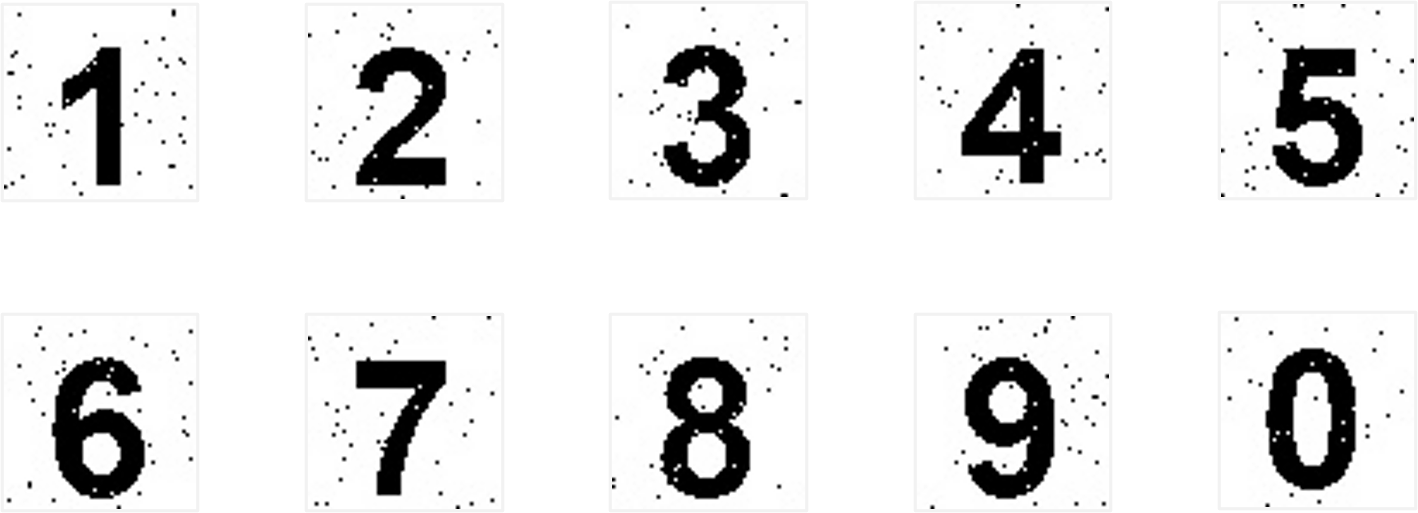
\includegraphics[width=.4\textwidth]{figuras/digitos_input.png}
    \caption{Exemplos de imagens $X$ a serem processadas com os dígitos $0-9$ e ruído sal e pimenta.}
    \label{fig:dig_X}
\end{figure}

\begin{figure}
    \centering
    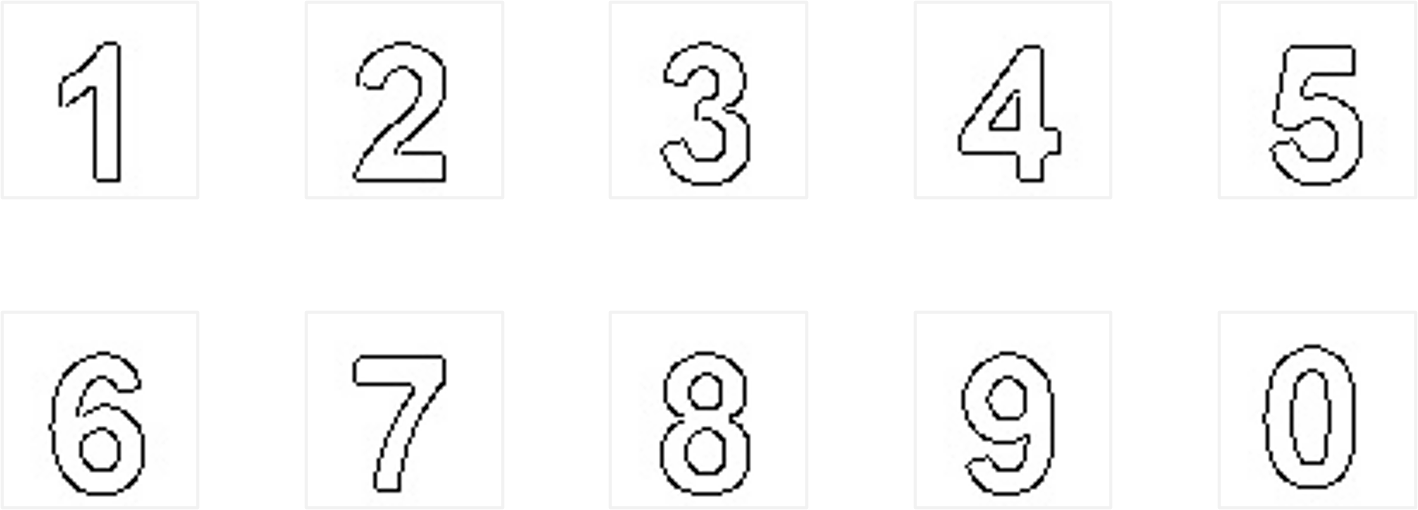
\includegraphics[width=.4\textwidth]{figuras/digitos_target.png}
    \caption{Exemplos de imagens $Y$ ideais com as bordas dos dígitos $0-9$ sem ruído.}
    \label{fig:dig_Y}
\end{figure}

Foram testadas diversas combinações de parâmetros para avaliar o desempenho do modelo, com a minimização do erro IoU, utilizando uma arquitetura de duas camadas ($n = 2$) e janelas 3x3 ($d_{W} = 3$). Os experimentos consideraram amostras de treinamento de 10 ou 30 imagens ($N = 10 \text{ ou } 30$) e amostras de validação de 10 imagens ($M = 10$). Para o reticulado das funções característica, foram amostrados 8 ou 16 vizinhos ($r = 8 \text{ ou } 16$), e para o reticulado da janela, 5 ou 9 vizinhos ($s = 5 \text{ ou } 9$). O processo de aprendizado da função característica foi conduzido por 100 épocas ($Epoch_f = 100$), enquanto o aprendizado da janela ocorreu por 50 épocas ($Epoch_w = 50$).

O tamanho do batch (batch size) variou de acordo com a quantidade de amostras de treinamento: batch de 5 ou 10 quando $N = 10$, e batch de 15 ou 30 quando $N = 30$. Para o critério de early stopping, foram utilizadas 30 épocas para o reticulado da função ($es_{f} = 30$) e 20 épocas para o reticulado da janela ($es_{w} = 20$). As janelas iniciais foram configuradas com uma estrutura em cruz ou com apenas o ponto central ativado ($W_{ini} = [[0,1,0],[1,1,1],[0,1,0]] \text{ ou } W_{ini} = [[0,0,0],[0,1,0],[0,0,0]]$). Todas essas configurações foram testadas de forma exaustiva, com variações feitas no esquema "todas contra todas", em que apenas um dos parâmetros era alterado por vez, mantendo os demais constantes.

Adicionalmente, foram realizados experimentos com uma única camada ($n = 1$), utilizando janelas 3x3 e 5x5 ($d_{W} = 3 \text{ ou } 5$), configuradas com os valores máximos para tamanho da amostra de treinamento, número de vizinhos amostrados, batch size e a janela inicial em cruz ($N = 30, r = 16, s = 9, b = 30, W_{ini} = [[0,1,0],[1,1,1],[0,1,0]]$), mantendo os demais parâmetros idênticos aos experimentos anteriores. Optou-se por não explorar extensivamente as combinações de parâmetros para uma única camada, dado que, devido à complexidade da solução, já se previa um desempenho inferior em comparação com as soluções de duas camadas. Esses experimentos serviram principalmente para evidenciar essa hipótese inicial.

Cada configuração de hiperparâmetros foi executada em uma \textit{run}, e cada \textit{run} foi repetida 10 vezes, alterando o parâmetro \textit{seed}. A \textit{seed} é um valor inicial que define a sequência de números produzidos pelo gerador de números aleatórios. Manter a mesma \textit{seed} e os mesmos parâmetros garante que, apesar da aleatoriedade inerente, os resultados sejam reprodutíveis. Portanto, considerar várias \textit{runs} com diferentes \textit{seeds} fornece uma visão mais robusta e confiável do desempenho do algoritmo sob diferentes condições de aleatoriedade.

Na Tabela \ref{tab:resultados_runs_digitos}, apresentamos os 10 melhores resultados das diferentes \textit{runs} ($R$). A tabela inclui os erros de treinamento ($L_{t}$), validação ($L_{v}$) e teste ($L_{tt}$) utilizando a notação "Valor Mínimo - Valor Médio (Desvio Padrão)". Ao final de cada execução calculou-se o erro de teste para cada uma das 10 \textit{seeds}, onde chegamos então no valor de erro de teste mínimo, médio e desvio padrão. Esse cálculo não teve interferência alguma nos treinamentos executados. Na tabela também temos a mínima época ($Epoch_{W_{min}}$ - época que obteve o menor erro de validação), os tempos em minutos de execução total de cada \textit{run} ($t_{total}$),  e o tempo para a mínima época ($t_{Epoch_{min}}$), estes também com a notação "Valor Mínimo - Valor Médio (Desvio Padrão)". Esses resultados fornecem uma visão abrangente do desempenho do algoritmo sob diferentes configurações de hiperparâmetros e \textit{seeds}. O critério de seleção das 10 melhores execuções foi: selecionar os 10 menores erros médios de teste e ordena-los pelo tempo de execução médio total. 

Na Tabela \ref{tab:hiperparametros_run} temos as configurações dos hiperparâmetros para cada uma das \textit{runs} selecionadas. A coluna $R$ indica cada \textit{run} da execução; $n$ é o número de camadas; $d_{W}$ é o tamanho da janela, $N$ e $M$ os tamanhos das amostras de treinamento e validação, respectivamente; $r$ e $s$ o número de vizinhos sorteados nos reticulados das funções característica e da janela, respectivamente; $Epoch_f$ e $Epoch_w$ as quantidade de épocas nos reticulados das funções característica e da janela, respectivamente; $b$ o tamanho do \textit{batch}; $es_f$ e $es_w$ os parâmetros de \textit{early stop} nos reticulados das funções característica e da janela, respectivamente; por fim, $W_{ini}$ é a configuração inicial dos W-operadores. 

No Apêndice \ref{apsec:reslts_digits} encontramos as tabelas \ref{tab:ap_resultados_runs_digitos} e \ref{tab:ap_hiperparametros_run} com os resultados completos de todas as execuções para esse experimento.

\begin{table}[ht]
    \centering
    \resizebox{\textwidth}{!}{ % Redimensiona a tabela para caber na largura da página
        \begin{tabular}{ccccccc}
            \toprule
            $R$ & $L_{t}$ & $L_{v}$ & $L_{tt}$ & $Epoch_{W_{min}}$ & $t_{total} \ (min)$ & $t_{Epoch_{min}} \ (min)$ \\
            \midrule
            17 & 0.0185 - 0.0757 (0.1405) & 0.0224 - 0.0775 (0.1397) & 0.0121 - 0.0167 (0.0023) & 13 - 29 (10) & 8.69 - 12.73 (1.91) & 2.63 - 7.45 (3.15) \\
            31 & 0.0195 - 0.0716 (0.1394) & 0.0227 - 0.0740 (0.1385) & 0.0128 - 0.0161 (0.0015) & 13 - 21 (7) & 9.60 - 13.53 (2.63) & 2.94 - 6.32 (2.54) \\
            16 & 0.0205 - 0.0371 (0.0297) & 0.0216 - 0.0384 (0.0292) & 0.0125 - 0.0152 (0.0017) & 12 - 30 (10) & 10.25 - 13.79 (1.53) & 3.51 - 8.64 (2.95) \\
            22 & 0.0209 - 0.0378 (0.0377) & 0.0217 - 0.0388 (0.0372) & 0.0124 - 0.0170 (0.0037) & 14 - 27 (11) & 11.06 - 15.26 (2.24) & 4.51 - 9.38 (3.95) \\
            25 & 0.0177 - 0.0708 (0.1398) & 0.0209 - 0.0729 (0.1389) & 0.0101 - 0.0156 (0.0030) & 20 - 33 (10) & 14.23 - 16.91 (1.49) & 5.32 - 11.00 (4.19) \\
            24 & 0.0173 - 0.0352 (0.0314) & 0.0203 - 0.0373 (0.0307) & 0.0110 - 0.0158 (0.0030) & 12 - 34 (12) & 14.09 - 18.55 (2.22) & 4.82 - 12.92 (4.59) \\
            20 & 0.0202 - 0.0333 (0.0300) & 0.0214 - 0.0346 (0.0295) & 0.0134 - 0.0156 (0.0015) & 8 - 25 (10) & 12.66 - 20.93 (3.30) & 3.23 - 11.90 (4.69) \\
            21 & 0.0183 - 0.0678 (0.1379) & 0.0208 - 0.0691 (0.1372) & 0.0123 - 0.0151 (0.0022) & 20 - 36 (9) & 19.90 - 21.84 (1.34) & 8.05 - 15.72 (4.50) \\
            29 & 0.0181 - 0.0674 (0.1405) & 0.0196 - 0.0697 (0.1395) & 0.0123 - 0.0145 (0.0018) & 14 - 37 (12) & 15.96 - 26.21 (4.55) & 4.80 - 19.49 (7.77) \\
            28 & 0.0171 - 0.0309 (0.0302) & 0.0198 - 0.0332 (0.0296) & 0.0104 - 0.0146 (0.0017) & 15 - 29 (10) & 19.92 - 27.70 (3.77) & 8.95 - 17.16 (6.07) \\

            \bottomrule
        \end{tabular}
    }
    \caption[Melhores 10 Runs experimentos dígitos]{Melhores 10 \textit{Runs}, cada uma com 10 execuções com \textit{seeds} diferentes. Erros IoU de treino, validação e teste, época que atingiu o menor erro de validação, tempos total e para atingir o menor erro de validação, calculados sob essas 10 execuções. Formato: Valor mínimo - Valor médio - Desvio padrão.}   
   % {Melhores 10 \textit{Runs}, cada uma com 10 execuções com \textit{seeds} diferentes. Erros IoU de treino, validação e teste, época que atingiu o menor erro de validação, tempos total e para atingir o menor erro de validação, calculados sob essas 10 execuções, no formato "Valor mínimo -- Valor médio (desvio padrão)".}
    \label{tab:resultados_runs_digitos}
\end{table}

\begin{table}[ht]
    \centering
    %\resizebox{\textwidth}{!}{ % Redimensiona a tabela para caber na largura da página
        \begin{tabular}{ccccccccccccc}
            \toprule
            $R$ & $n$ & $d_{w}$ & $N$ & $M$ & $r$ & $s$ & $Epoch_f$ & $Epoch_w$ & $b$ & $es_{f}$ & $es_{w}$ & $W_{ini}$ \\
            \midrule
            17 & 2 & 3 & 30 & 10 & 8 & 5 & 100 & 50 & 15 & 30 & 20 & Centro \\
            31 & 2 & 3 & 30 & 10 & 16 & 9 & 100 & 50 & 30 & 30 & 20 & Centro \\
            16 & 2 & 3 & 30 & 10 & 8 & 5 & 100 & 50 & 15 & 30 & 20 & Cruz \\
            22 & 2 & 3 & 30 & 10 & 8 & 9 & 100 & 50 & 30 & 30 & 20 & Cruz \\
            25 & 2 & 3 & 30 & 10 & 16 & 5 & 100 & 50 & 15 & 30 & 20 & Centro \\
            24 & 2 & 3 & 30 & 10 & 16 & 5 & 100 & 50 & 15 & 30 & 20 & Cruz \\
            20 & 2 & 3 & 30 & 10 & 8 & 9 & 100 & 50 & 15 & 30 & 20 & Cruz \\
            21 & 2 & 3 & 30 & 10 & 8 & 9 & 100 & 50 & 15 & 30 & 20 & Centro \\
            29 & 2 & 3 & 30 & 10 & 16 & 9 & 100 & 50 & 15 & 30 & 20 & Centro \\
            28 & 2 & 3 & 30 & 10 & 16 & 9 & 100 & 50 & 15 & 30 & 20 & Cruz \\
            \bottomrule
        \end{tabular}
   % }
    \caption[Configuração de hiperparâmetros das 10 melhores \textit{Runs} experimento dígitos]{Configuração de hiperparâmetros das 10 melhores \textit{Runs}: quantidade de camadas, tamanho da janela, tamanho da amostra de treinamento, tamanho da amostra de validação, quantidade de vizinhos do reticulado da função amostrados, quantidade de vizinhos no reticulado da janela amostrados, quantidade de épocas para o treinamento da função característica, quantidade de épocas para o treinamento da janela, tamanho do \textit{batch}, parâmetros de \textit{early stop} para os aprendizados da função e da janela, respectivamente e janela inicial de treinamento.}
    \label{tab:hiperparametros_run}
\end{table}

A análise das Tabelas \ref{tab:resultados_runs_digitos} e \ref{tab:hiperparametros_run}, que apresentam os resultados das 10 melhores execuções, demonstra de forma clara como a variação de diferentes hiperparâmetros influencia os erros e os tempos de execução. Observa-se que o aumento no tamanho da base de dados de treinamento ($N$) tende a favorecer uma melhor generalização do modelo. Este fato é evidenciado pelo fato de que todas as 10 melhores execuções utilizam o maior tamanho de amostra de treinamento testado (30 imagens). Além disso, o tamanho do \textit{batch} também mostrou ter uma influência significativa nos menores erros obtidos, com $80\%$ das execuções apresentando um \textit{batch} de tamanho $b=15$. \textit{Batches} menores permitem que o algoritmo percorra mais pontos do reticulado por época, o que contribui para uma busca mais eficaz pelo mínimo erro, além de escapar de regiões com alto erro. Por fim, a configuração com duas camadas de W-operadores 3x3 se destacou como a mais eficaz para esta solução, sendo consistentemente a escolhida em todas as 10 melhores execuções. Isso sugere que essa arquitetura de W-operadores multicamadas oferece um equilíbrio adequado entre complexidade e capacidade de captura de padrões relevantes, contribuindo de maneira decisiva para a obtenção dos melhores resultados.

Demais variações de hiperparâmetros, mantendo as configurações acima constantes, não produziram um impacto significativo no erro, mas afetaram consideravelmente o tempo de execução. Como esperado, o aumento no número de vizinhos sorteados nos reticulados tende a reduzir o erro, porém, à custa de um aumento substancial no tempo de execução. Por exemplo, ao comparar as execuções 17 e 28, observa-se que o erro médio de teste diminuiu de 0.0167 para 0.0146, representando uma redução de aproximadamente 12.6\%. Contudo, o tempo médio de execução aumentou de 12.73 minutos para 27.70 minutos, uma elevação de cerca de 117.6\%. Esse trade-off evidencia a necessidade de balancear a busca por menores erros com a eficiência computacional do algoritmo.

A Figura \ref{fig:validation_errors} apresenta os gráficos dos erros de validação ao longo das épocas do reticulado da janela para as seis execuções com menor erro médio. Cada subfigura representa uma execução específica corresponde aos parâmetros e resultados indicados nas tabelas \ref{tab:resultados_runs_digitos} e \ref{tab:hiperparametros_run}. As variações entre os gráficos refletem o impacto que diferentes seeds podem ter sobre o processo de treinamento com o mesmo parâmetro, especialmente em termos de convergência e minimização do erro de validação. Essa análise é fundamental para garantir que o modelo não apenas alcance um bom desempenho médio, mas também seja estável e confiável quando submetido a condições iniciais diferentes durante a fase de treinamento.

Outro ponto relevante a ser observado nos gráficos é a diferença significativa no erro inicial entre as execuções em que a janela inicial é o "Centro" (\textit{Runs} 21, 29 e 25) e aquelas em que a janela inicial é a "Cruz" (\textit{Runs} 16, 20 e 28). Nas execuções iniciadas com a janela "Centro", o erro inicial é substancialmente maior, o que impacta diretamente a quantidade de épocas necessárias para atingir o erro mínimo. Por exemplo, comparando as \textit{Runs} 28 e 29, observa-se um aumento de 29 para 37 épocas até encontrar o erro mínimo, o que representa um incremento de aproximadamente 27,6\% no número de épocas. Apesar desse aumento no número de épocas, o tempo médio de execução diminui de 27,70 para 26,21 minutos, uma redução de cerca de 5,4\%. Este fenômeno sugere que, embora o número de épocas da janela seja um fator importante, o algoritmo ainda depende do caminho no reticulado percorrido. No ponto inicial de cruz existe uma probabilidade maior de buscarmos em janelas mais complexas, inclusive a janela completa, que por consequência possui uma função característica maior e pode levar mais tempo na busca no reticulado da função.

\begin{figure}[H]
  \centering
  
  \begin{subfigure}{0.45\textwidth}
    \centering
    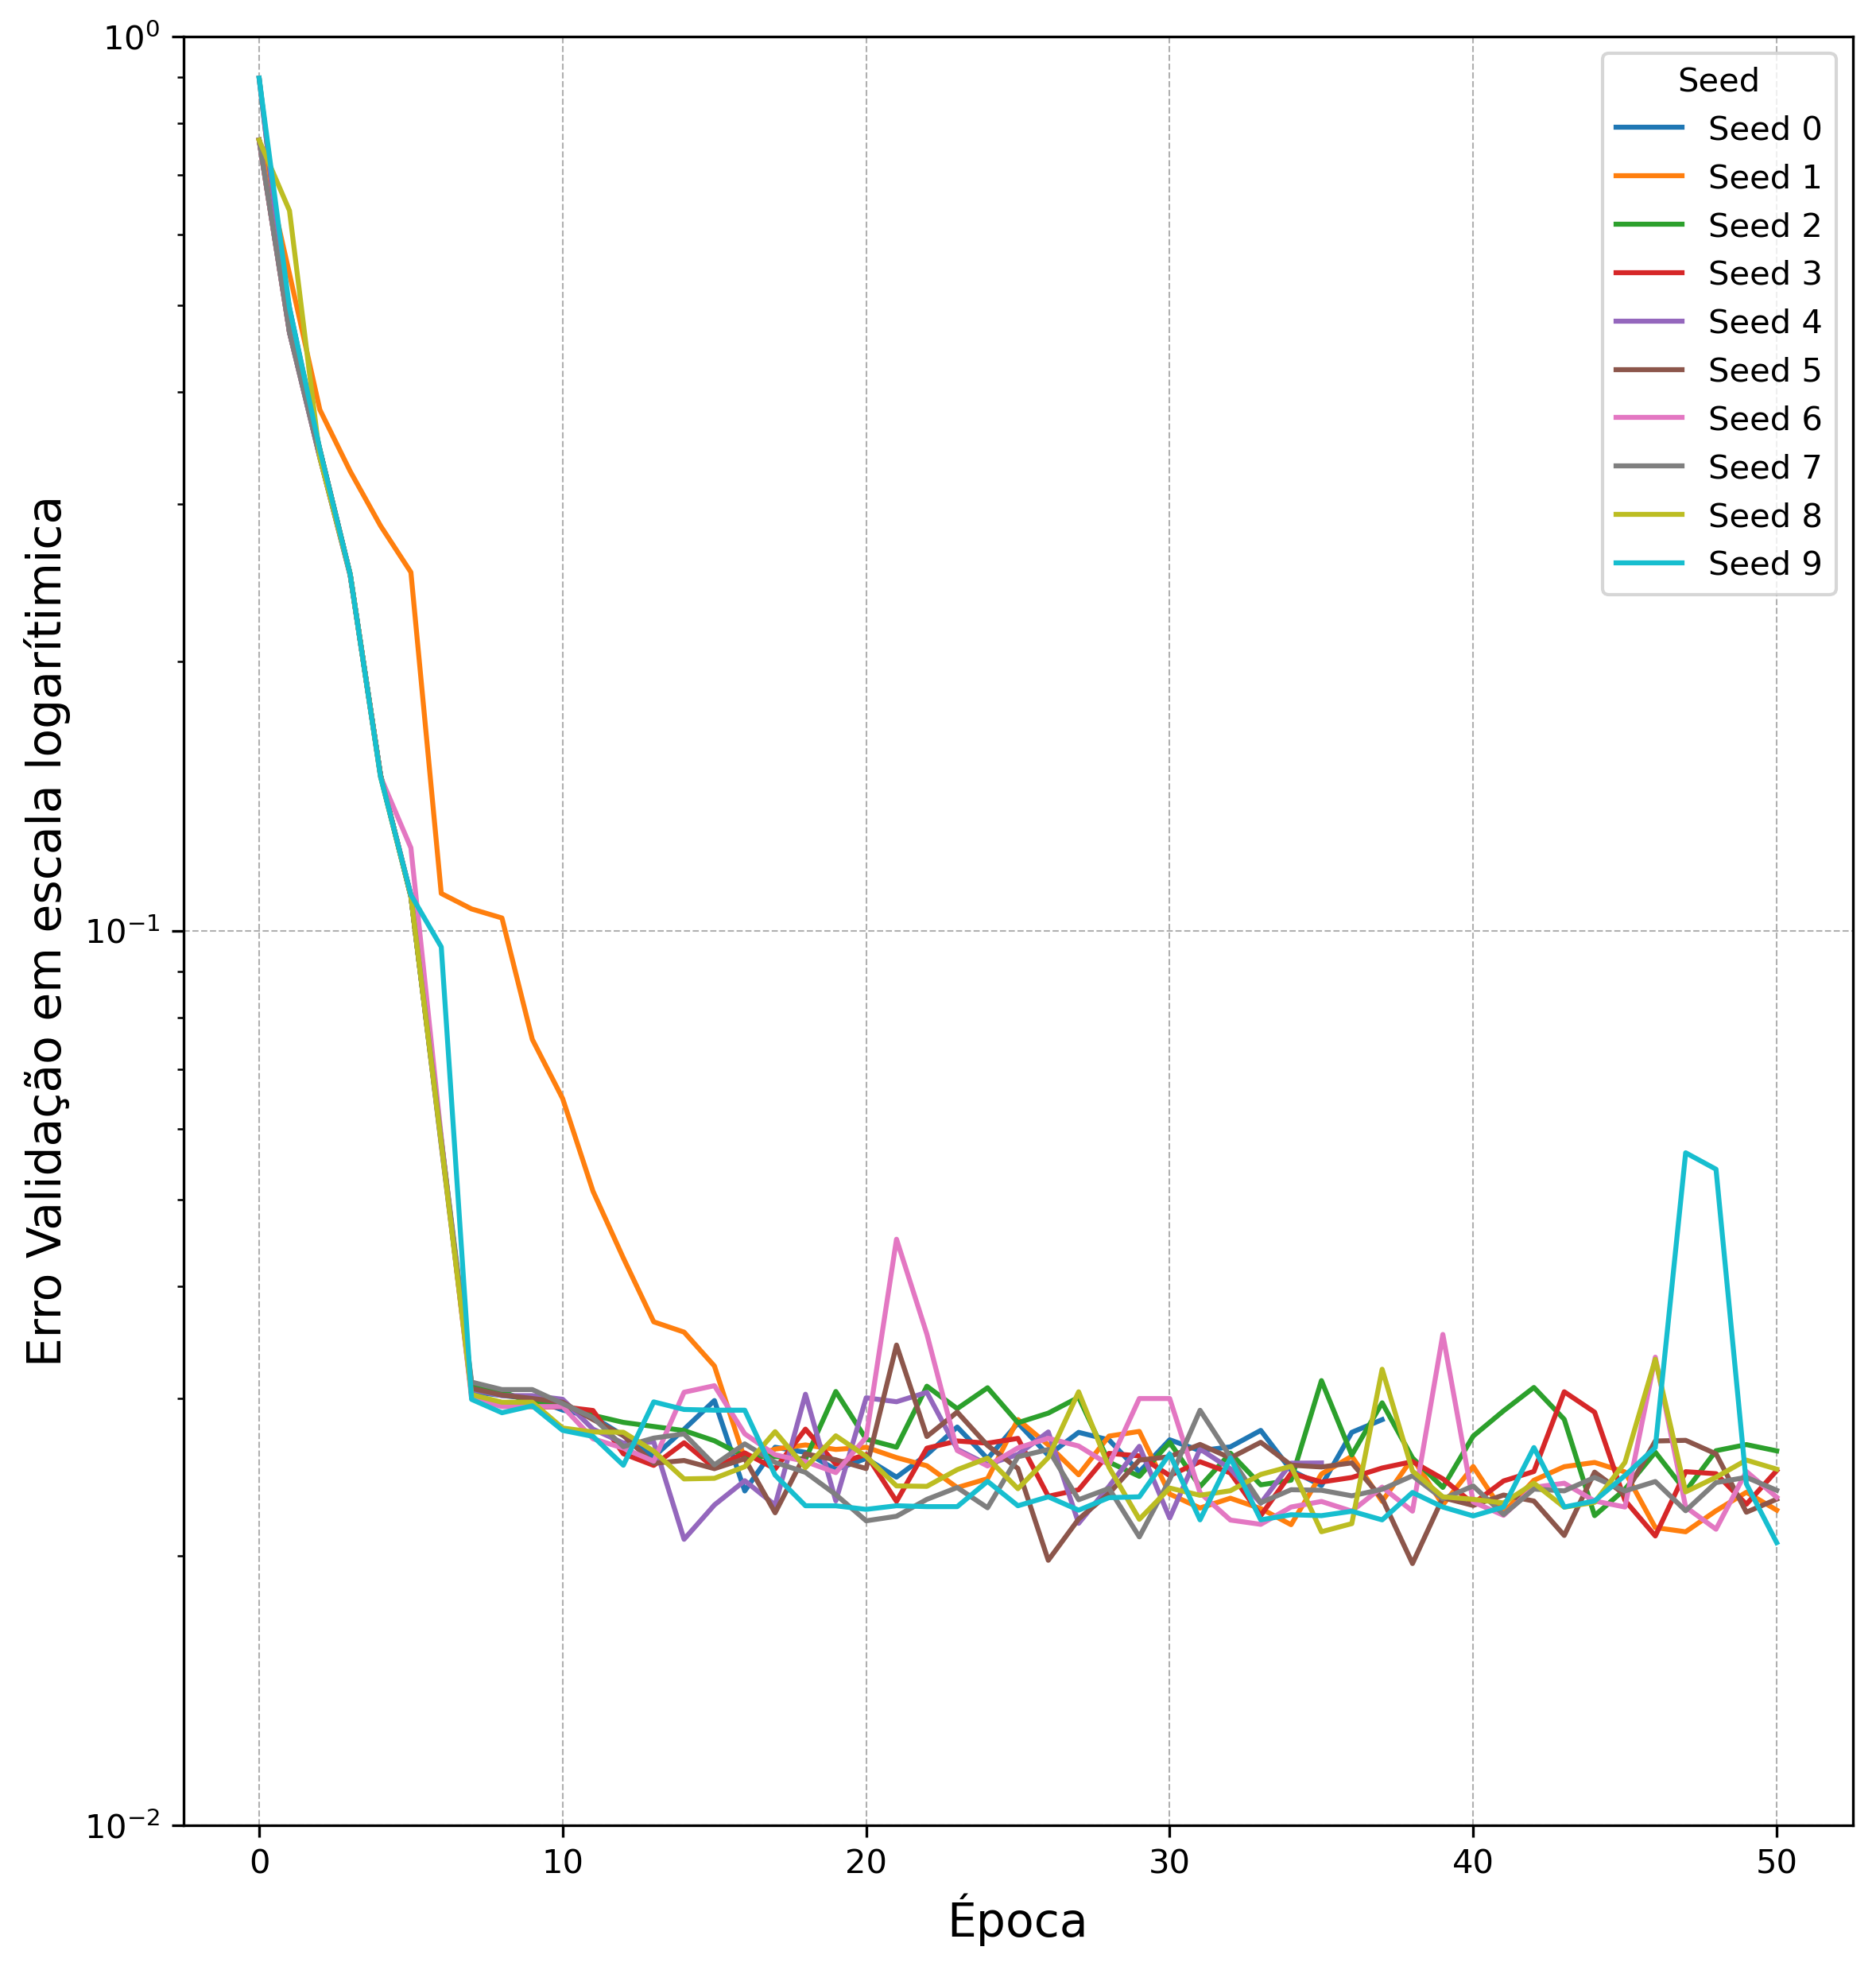
\includegraphics[width=\textwidth]{error_val_plot_29.png}
    \caption{Run 29 - $L_{tt_{mean}}=0.0145$}
  \end{subfigure}
  \hfill
  \begin{subfigure}{0.45\textwidth}
    \centering
    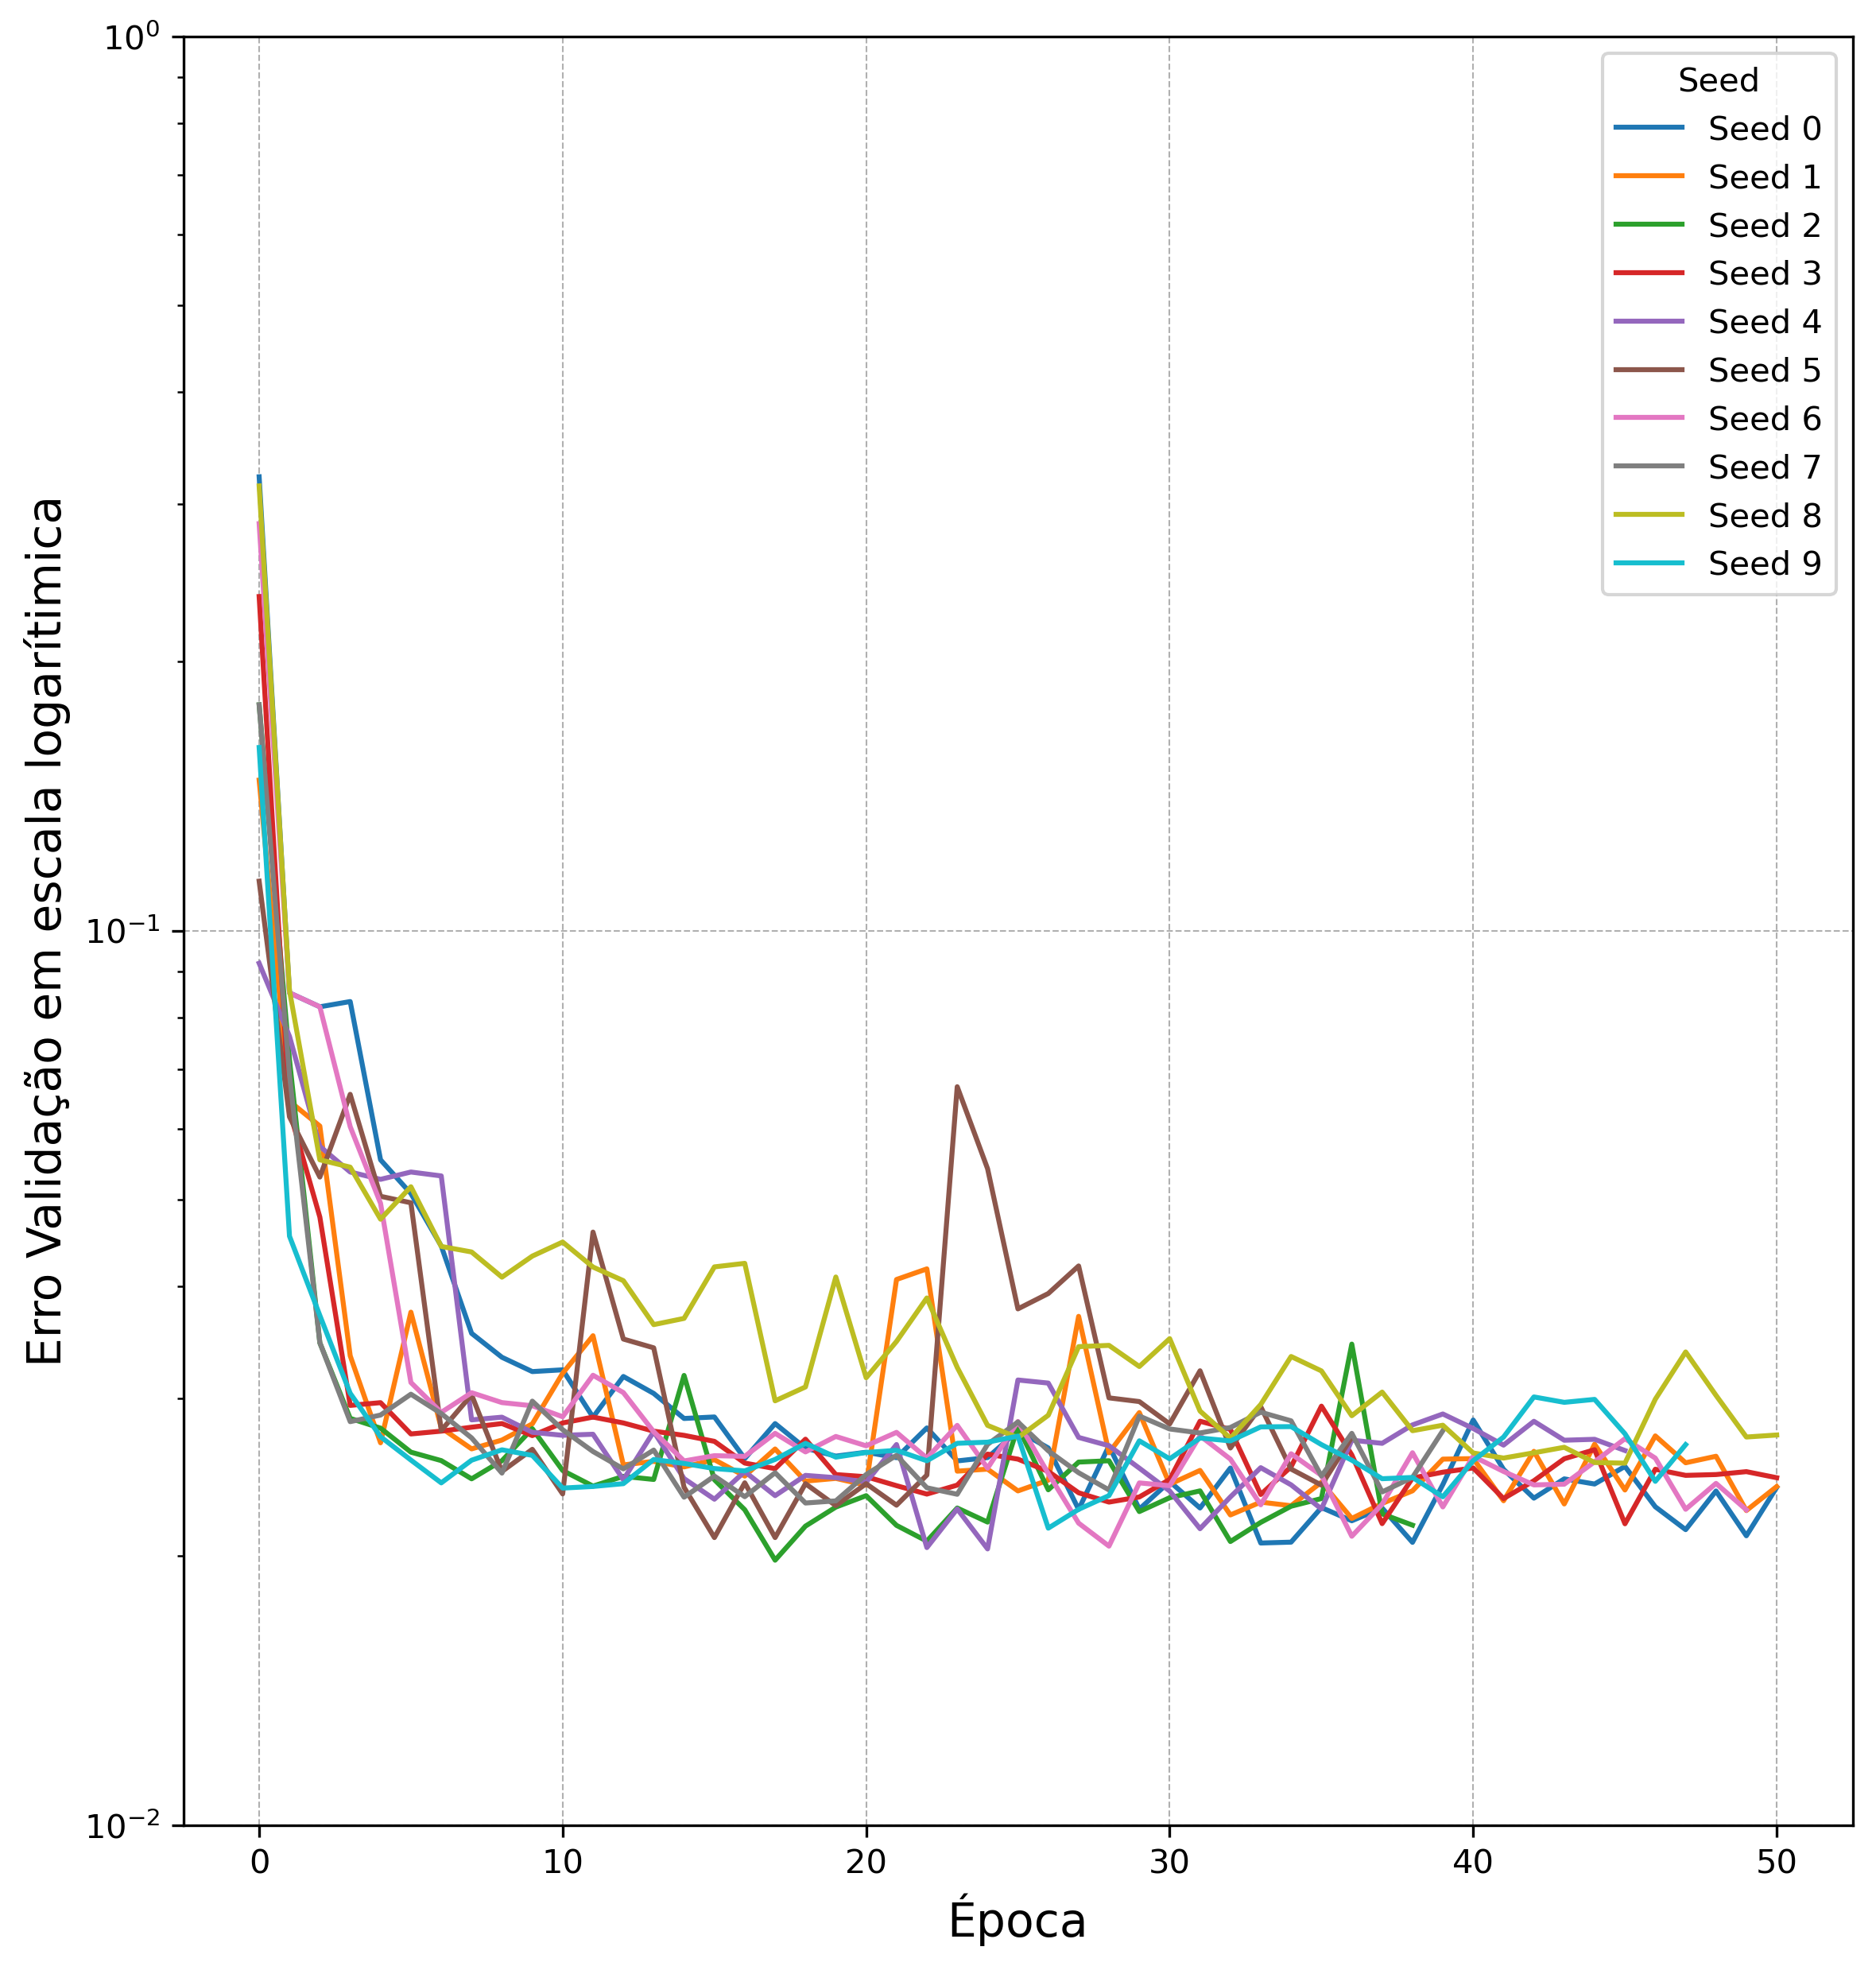
\includegraphics[width=\textwidth]{error_val_plot_28.png}
    \caption{Run 28 - $L_{tt_{mean}}=0.0146$}
  \end{subfigure}
  
  \vspace{0.3cm}
  
  \begin{subfigure}{0.45\textwidth}
    \centering
    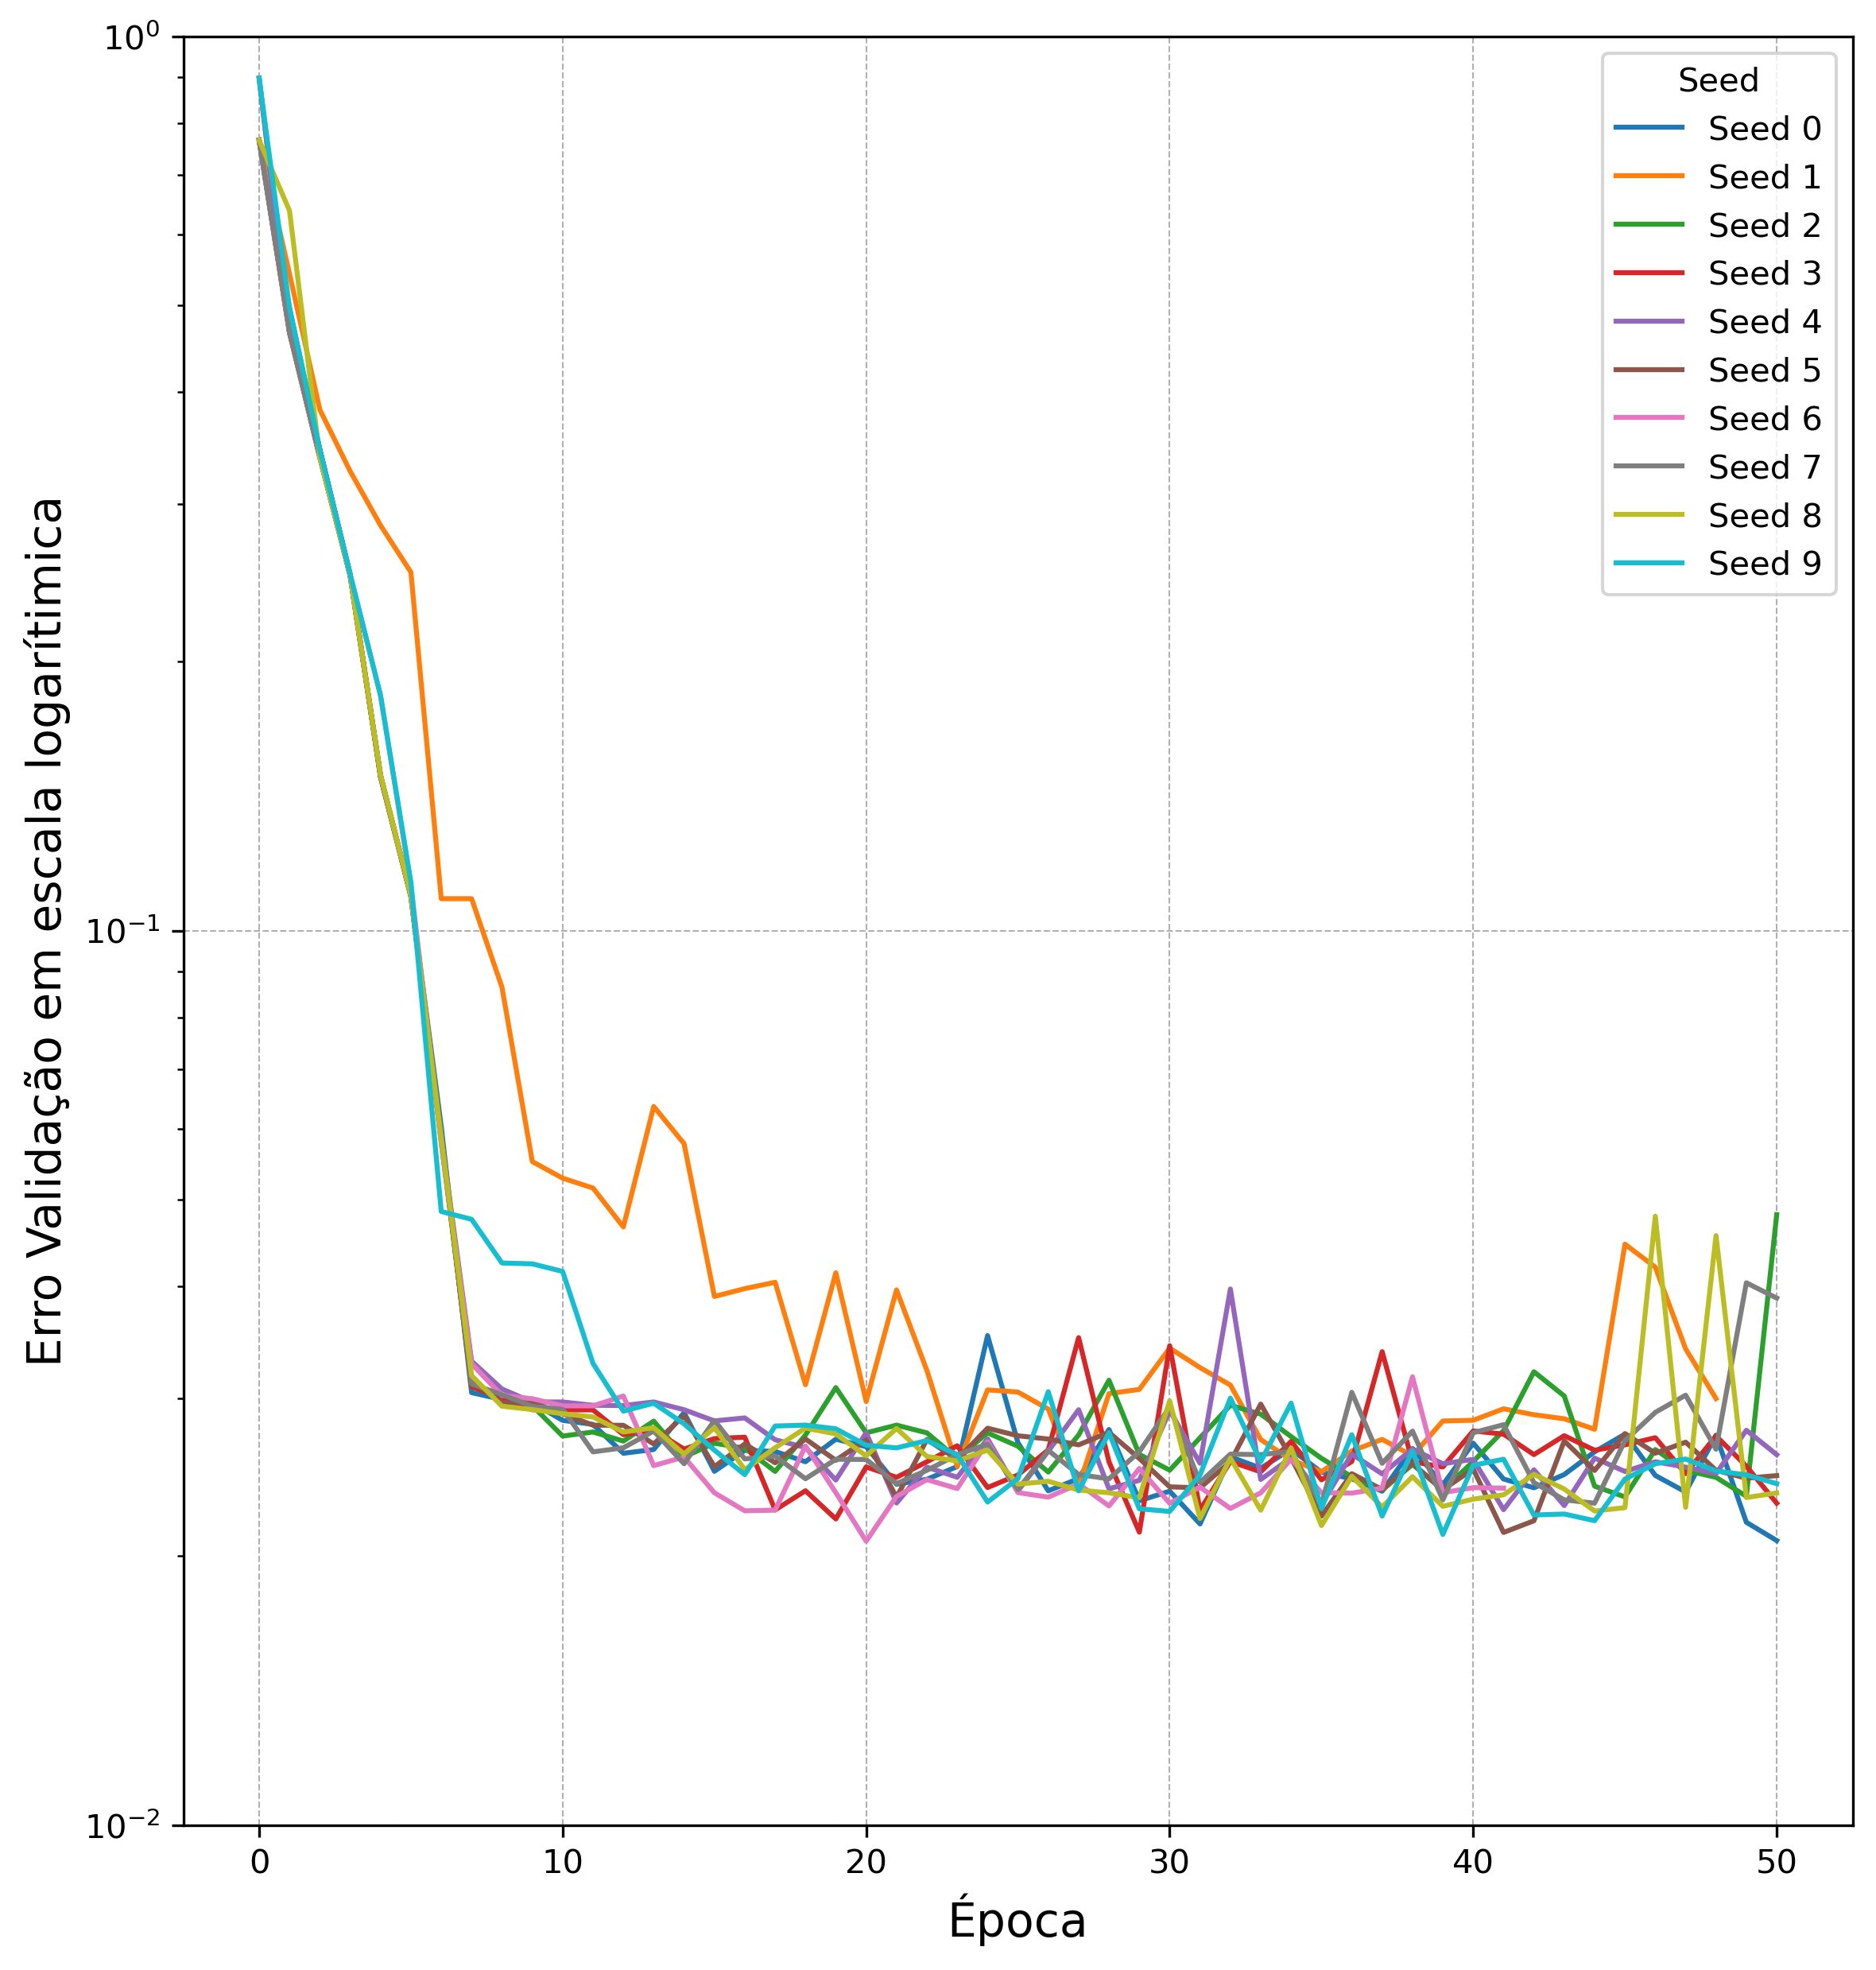
\includegraphics[width=\textwidth]{error_val_plot_21.png}
    \caption{Run 21 - $L_{tt_{mean}}=0.0151$}
  \end{subfigure}
  \hfill
  \begin{subfigure}{0.45\textwidth}
    \centering
    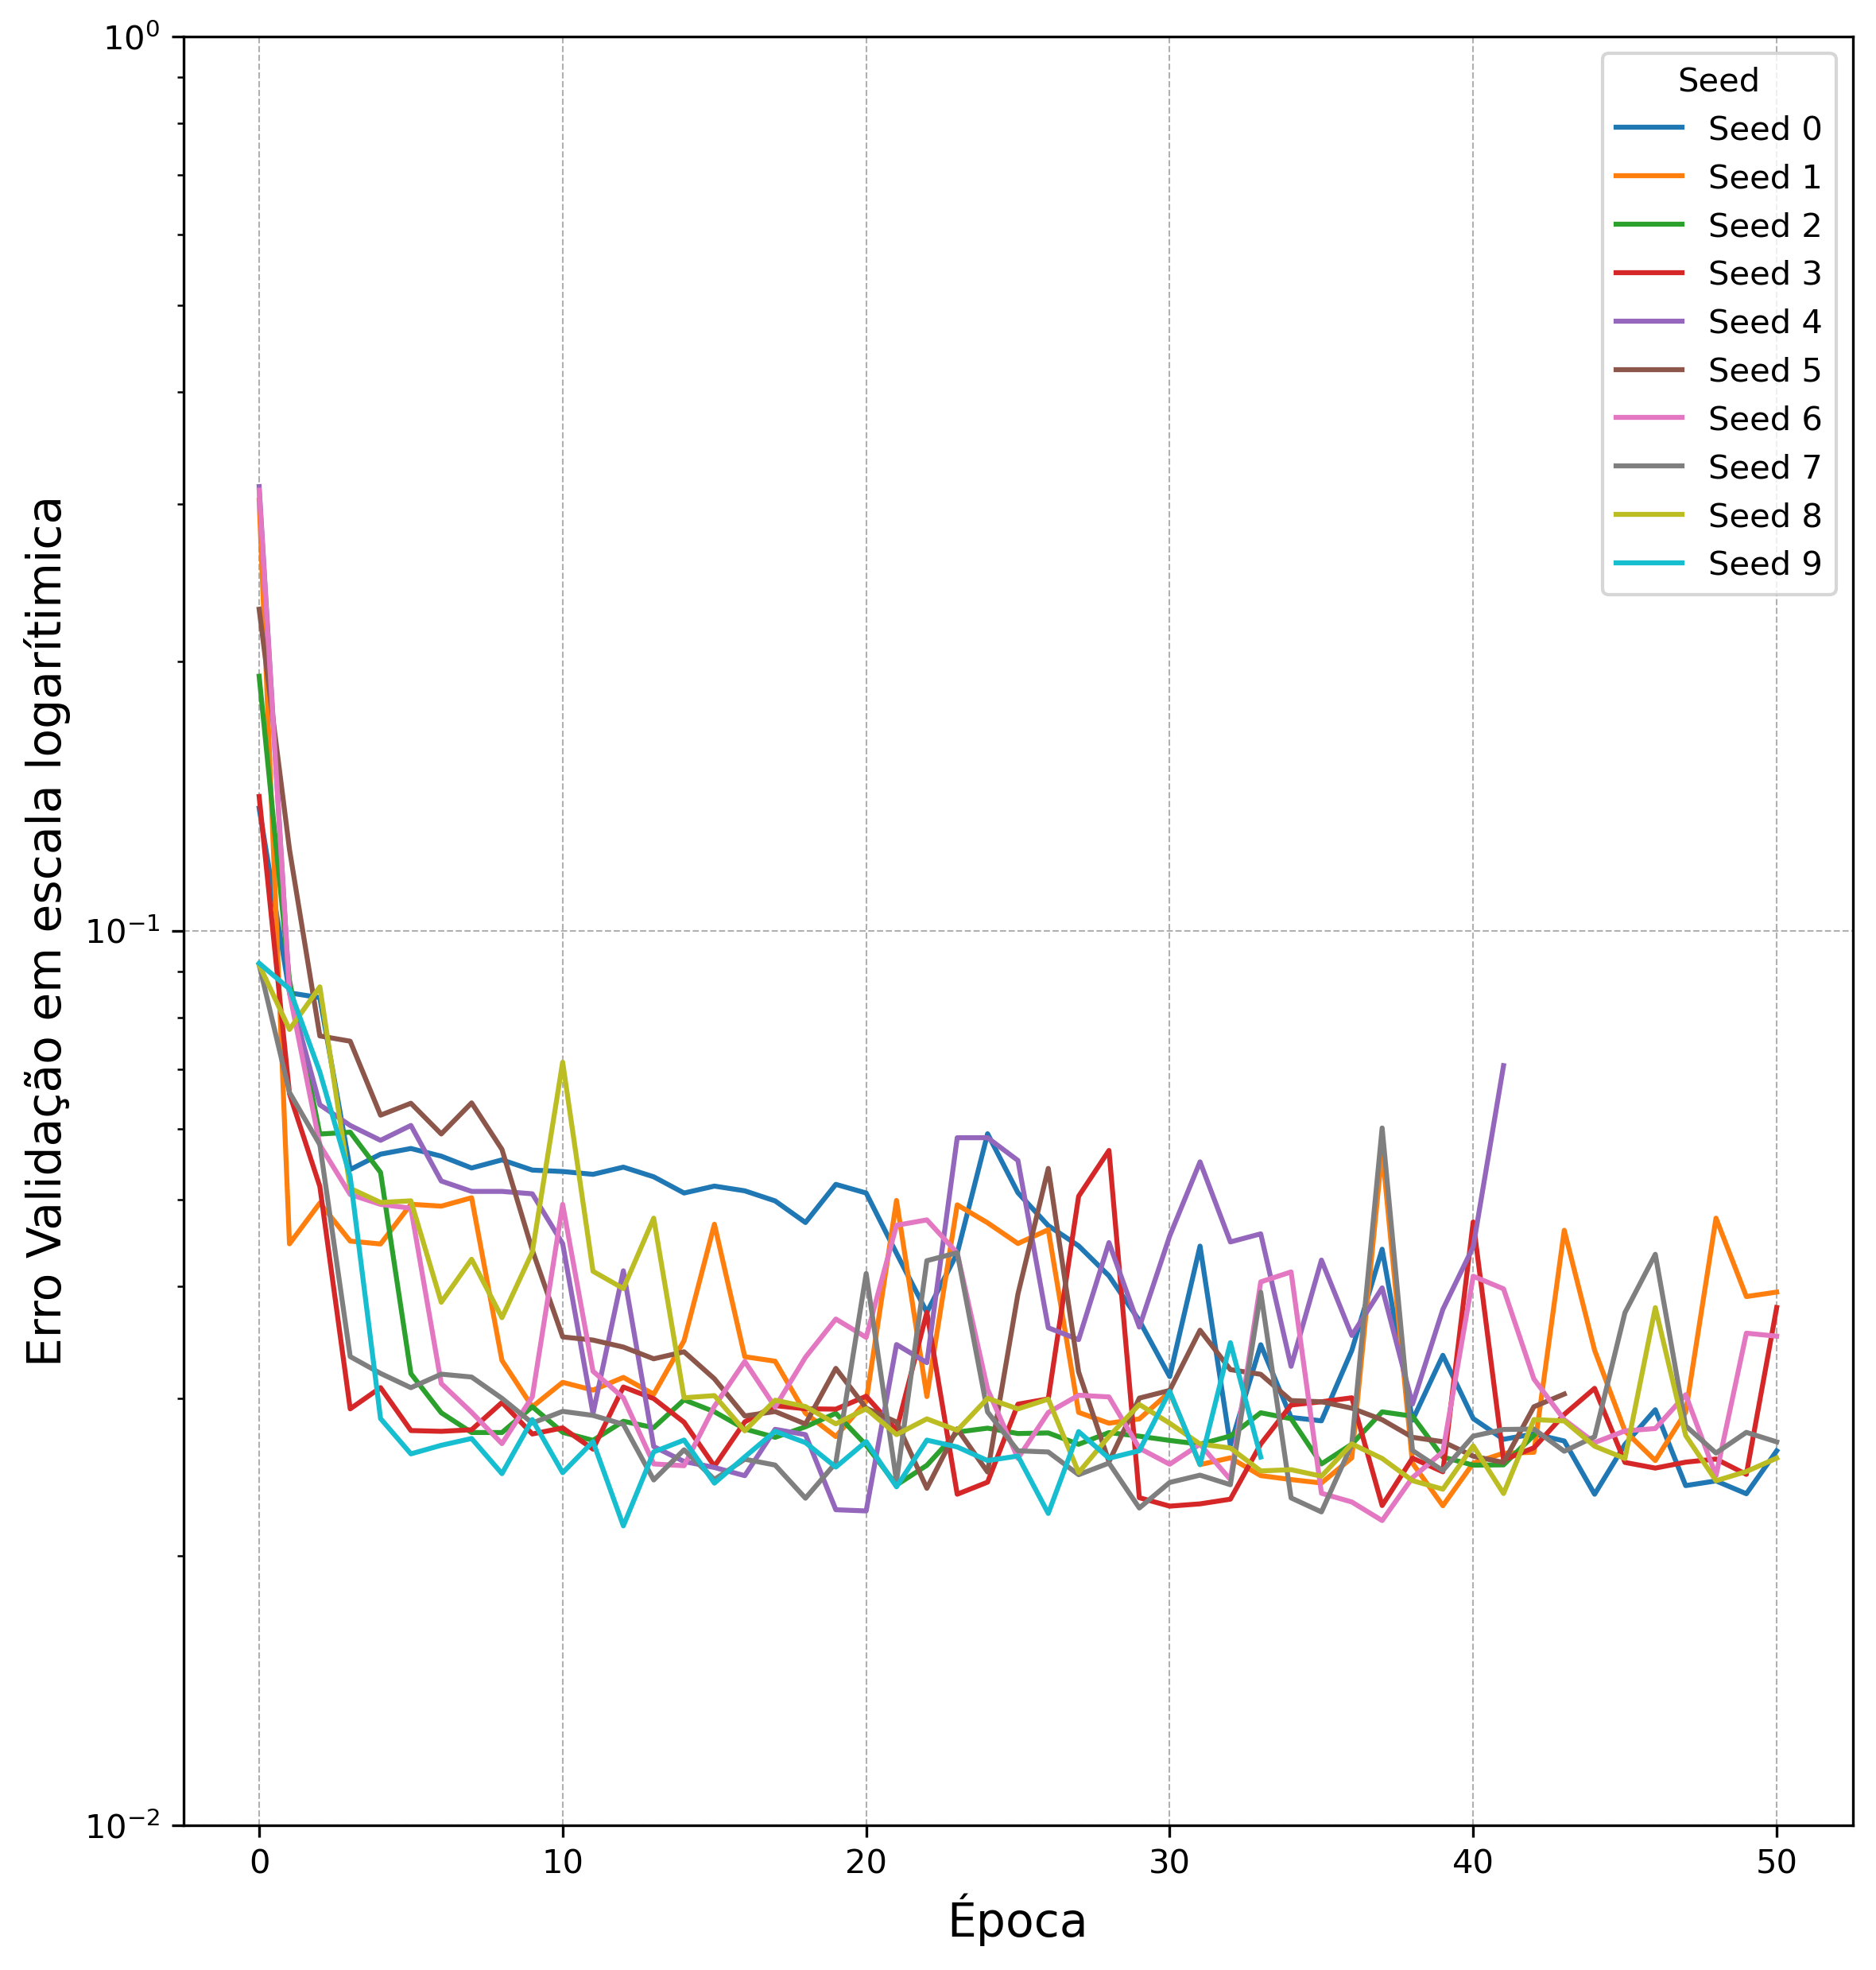
\includegraphics[width=\textwidth]{error_val_plot_16.png}
    \caption{Run 16 - $L_{tt_{mean}}=0.0152$}
  \end{subfigure}
  
  \vspace{0.3cm}
  
  \begin{subfigure}{0.45\textwidth}
    \centering
    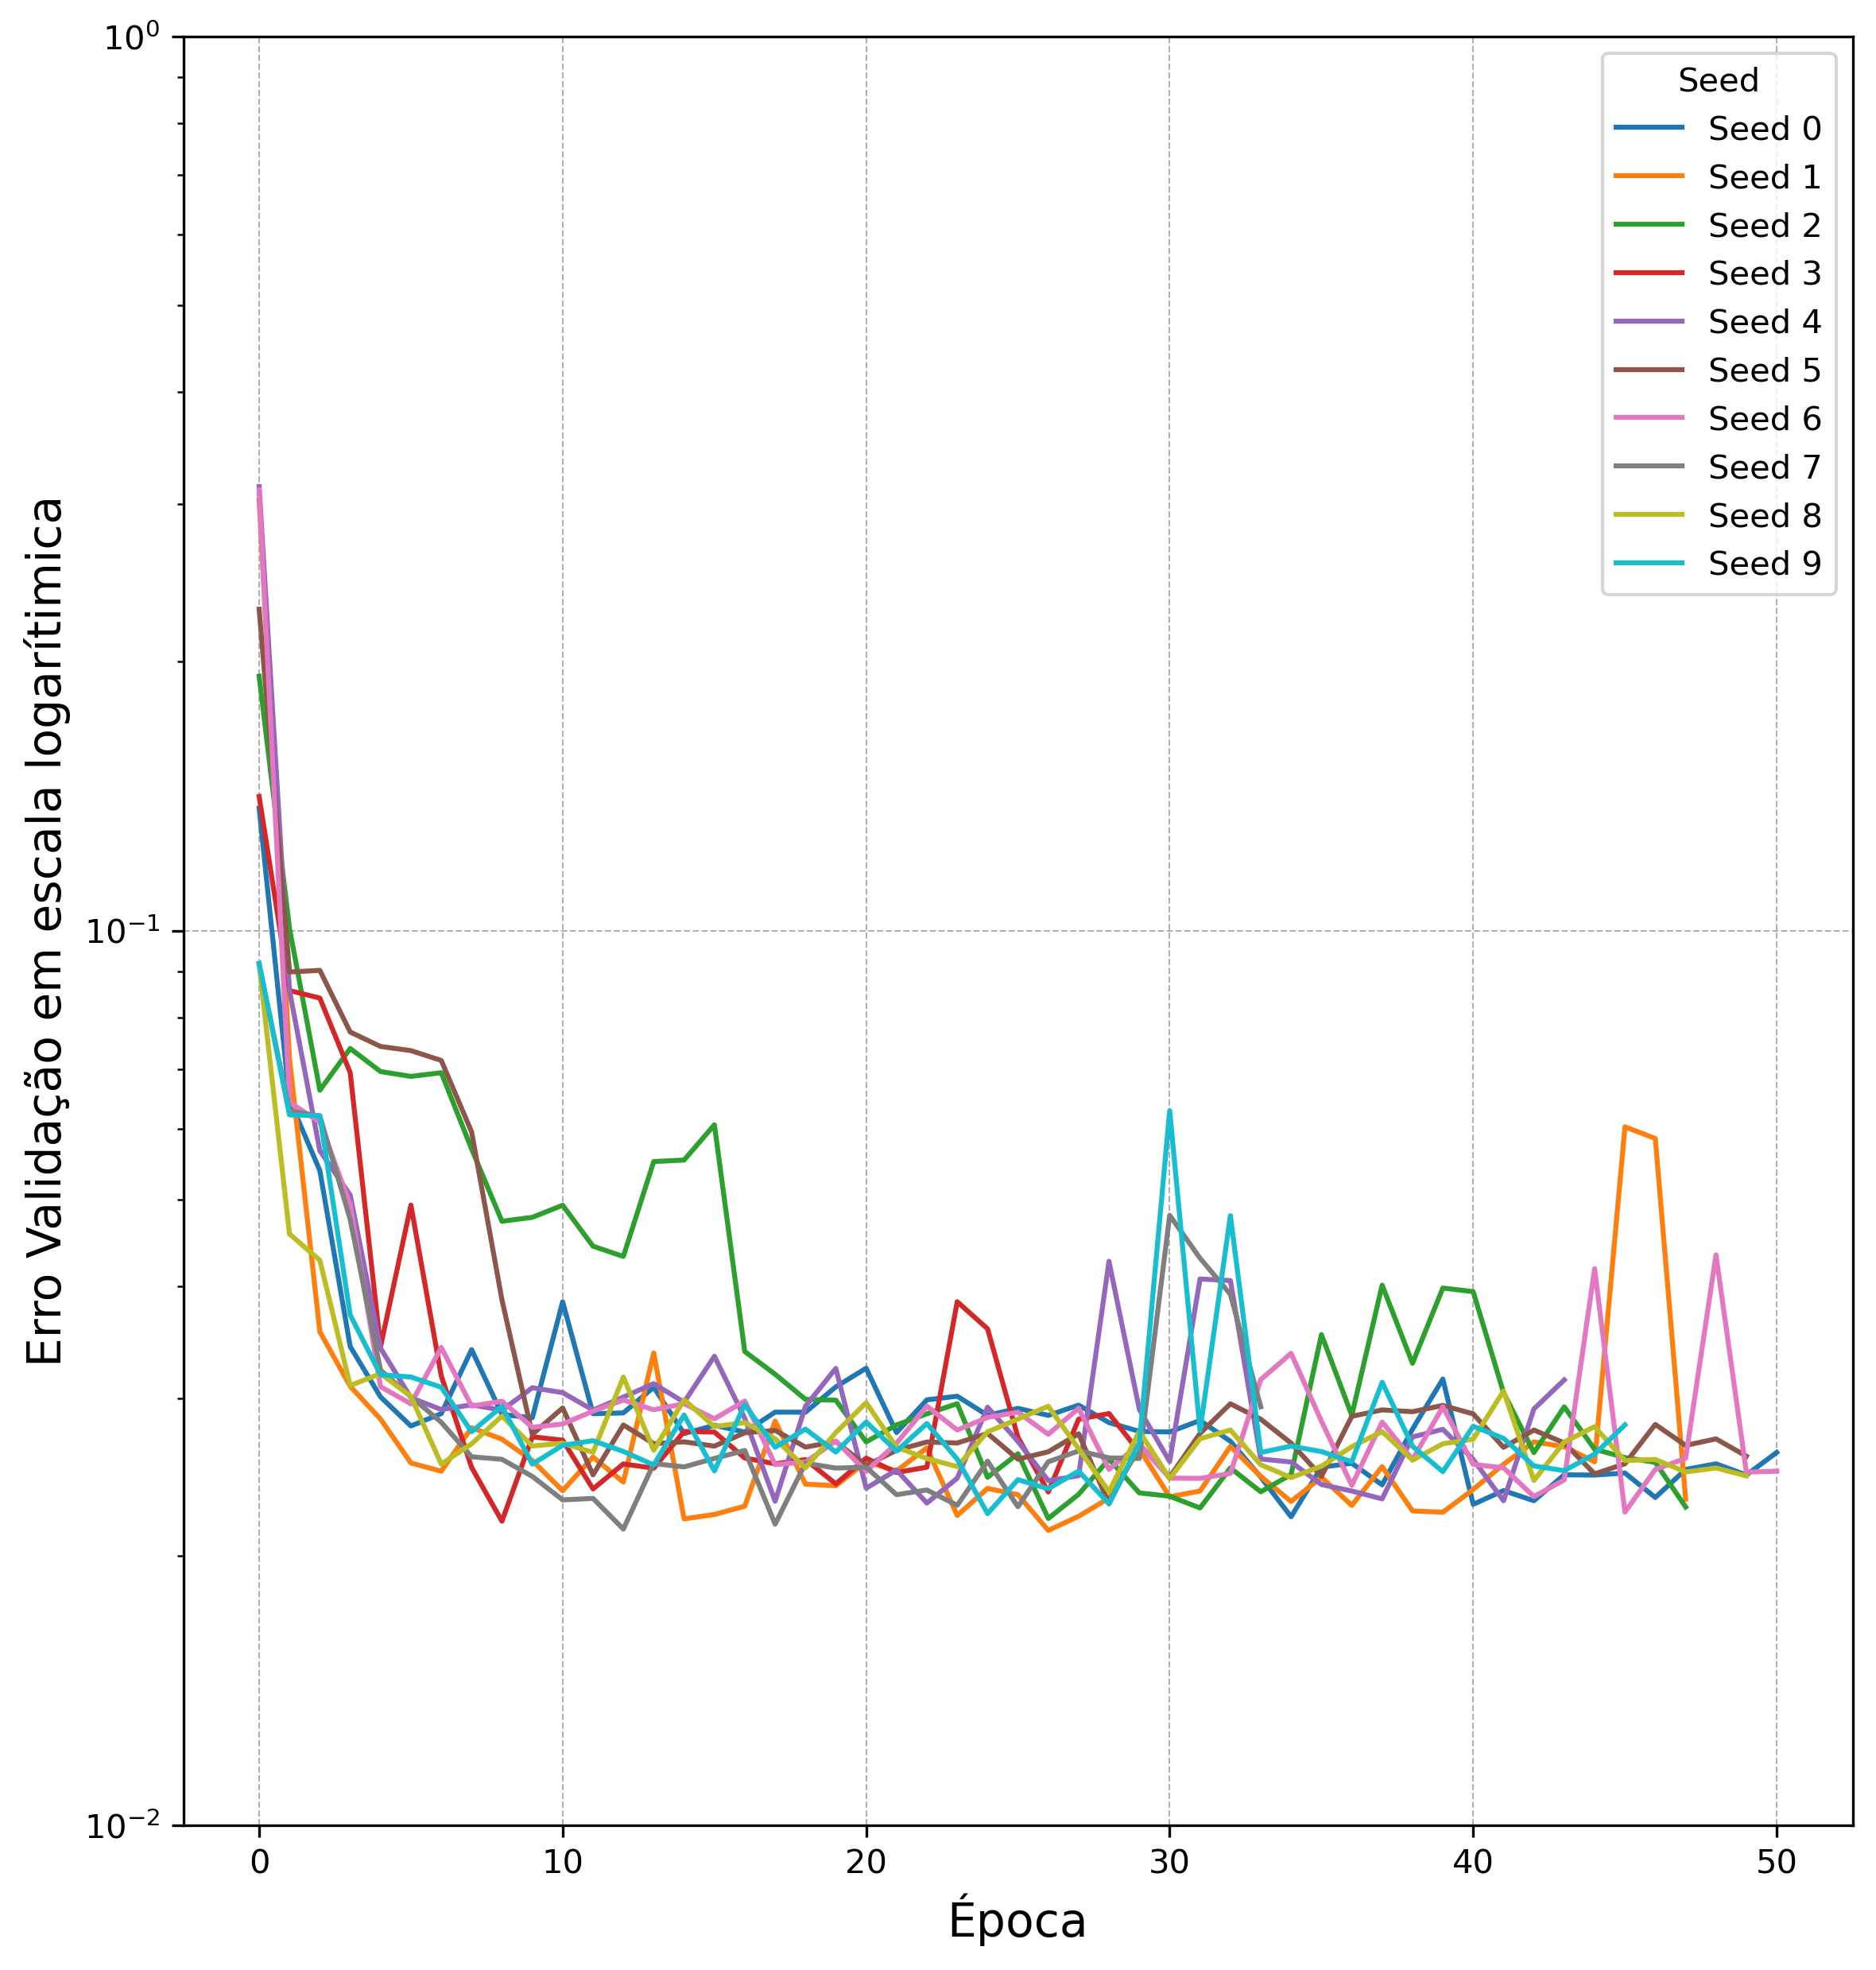
\includegraphics[width=\textwidth]{error_val_plot_20.png}
    \caption{Run 20 - $L_{tt_{mean}}=0.0156$}
  \end{subfigure}
  \hfill
  \begin{subfigure}{0.45\textwidth}
    \centering
    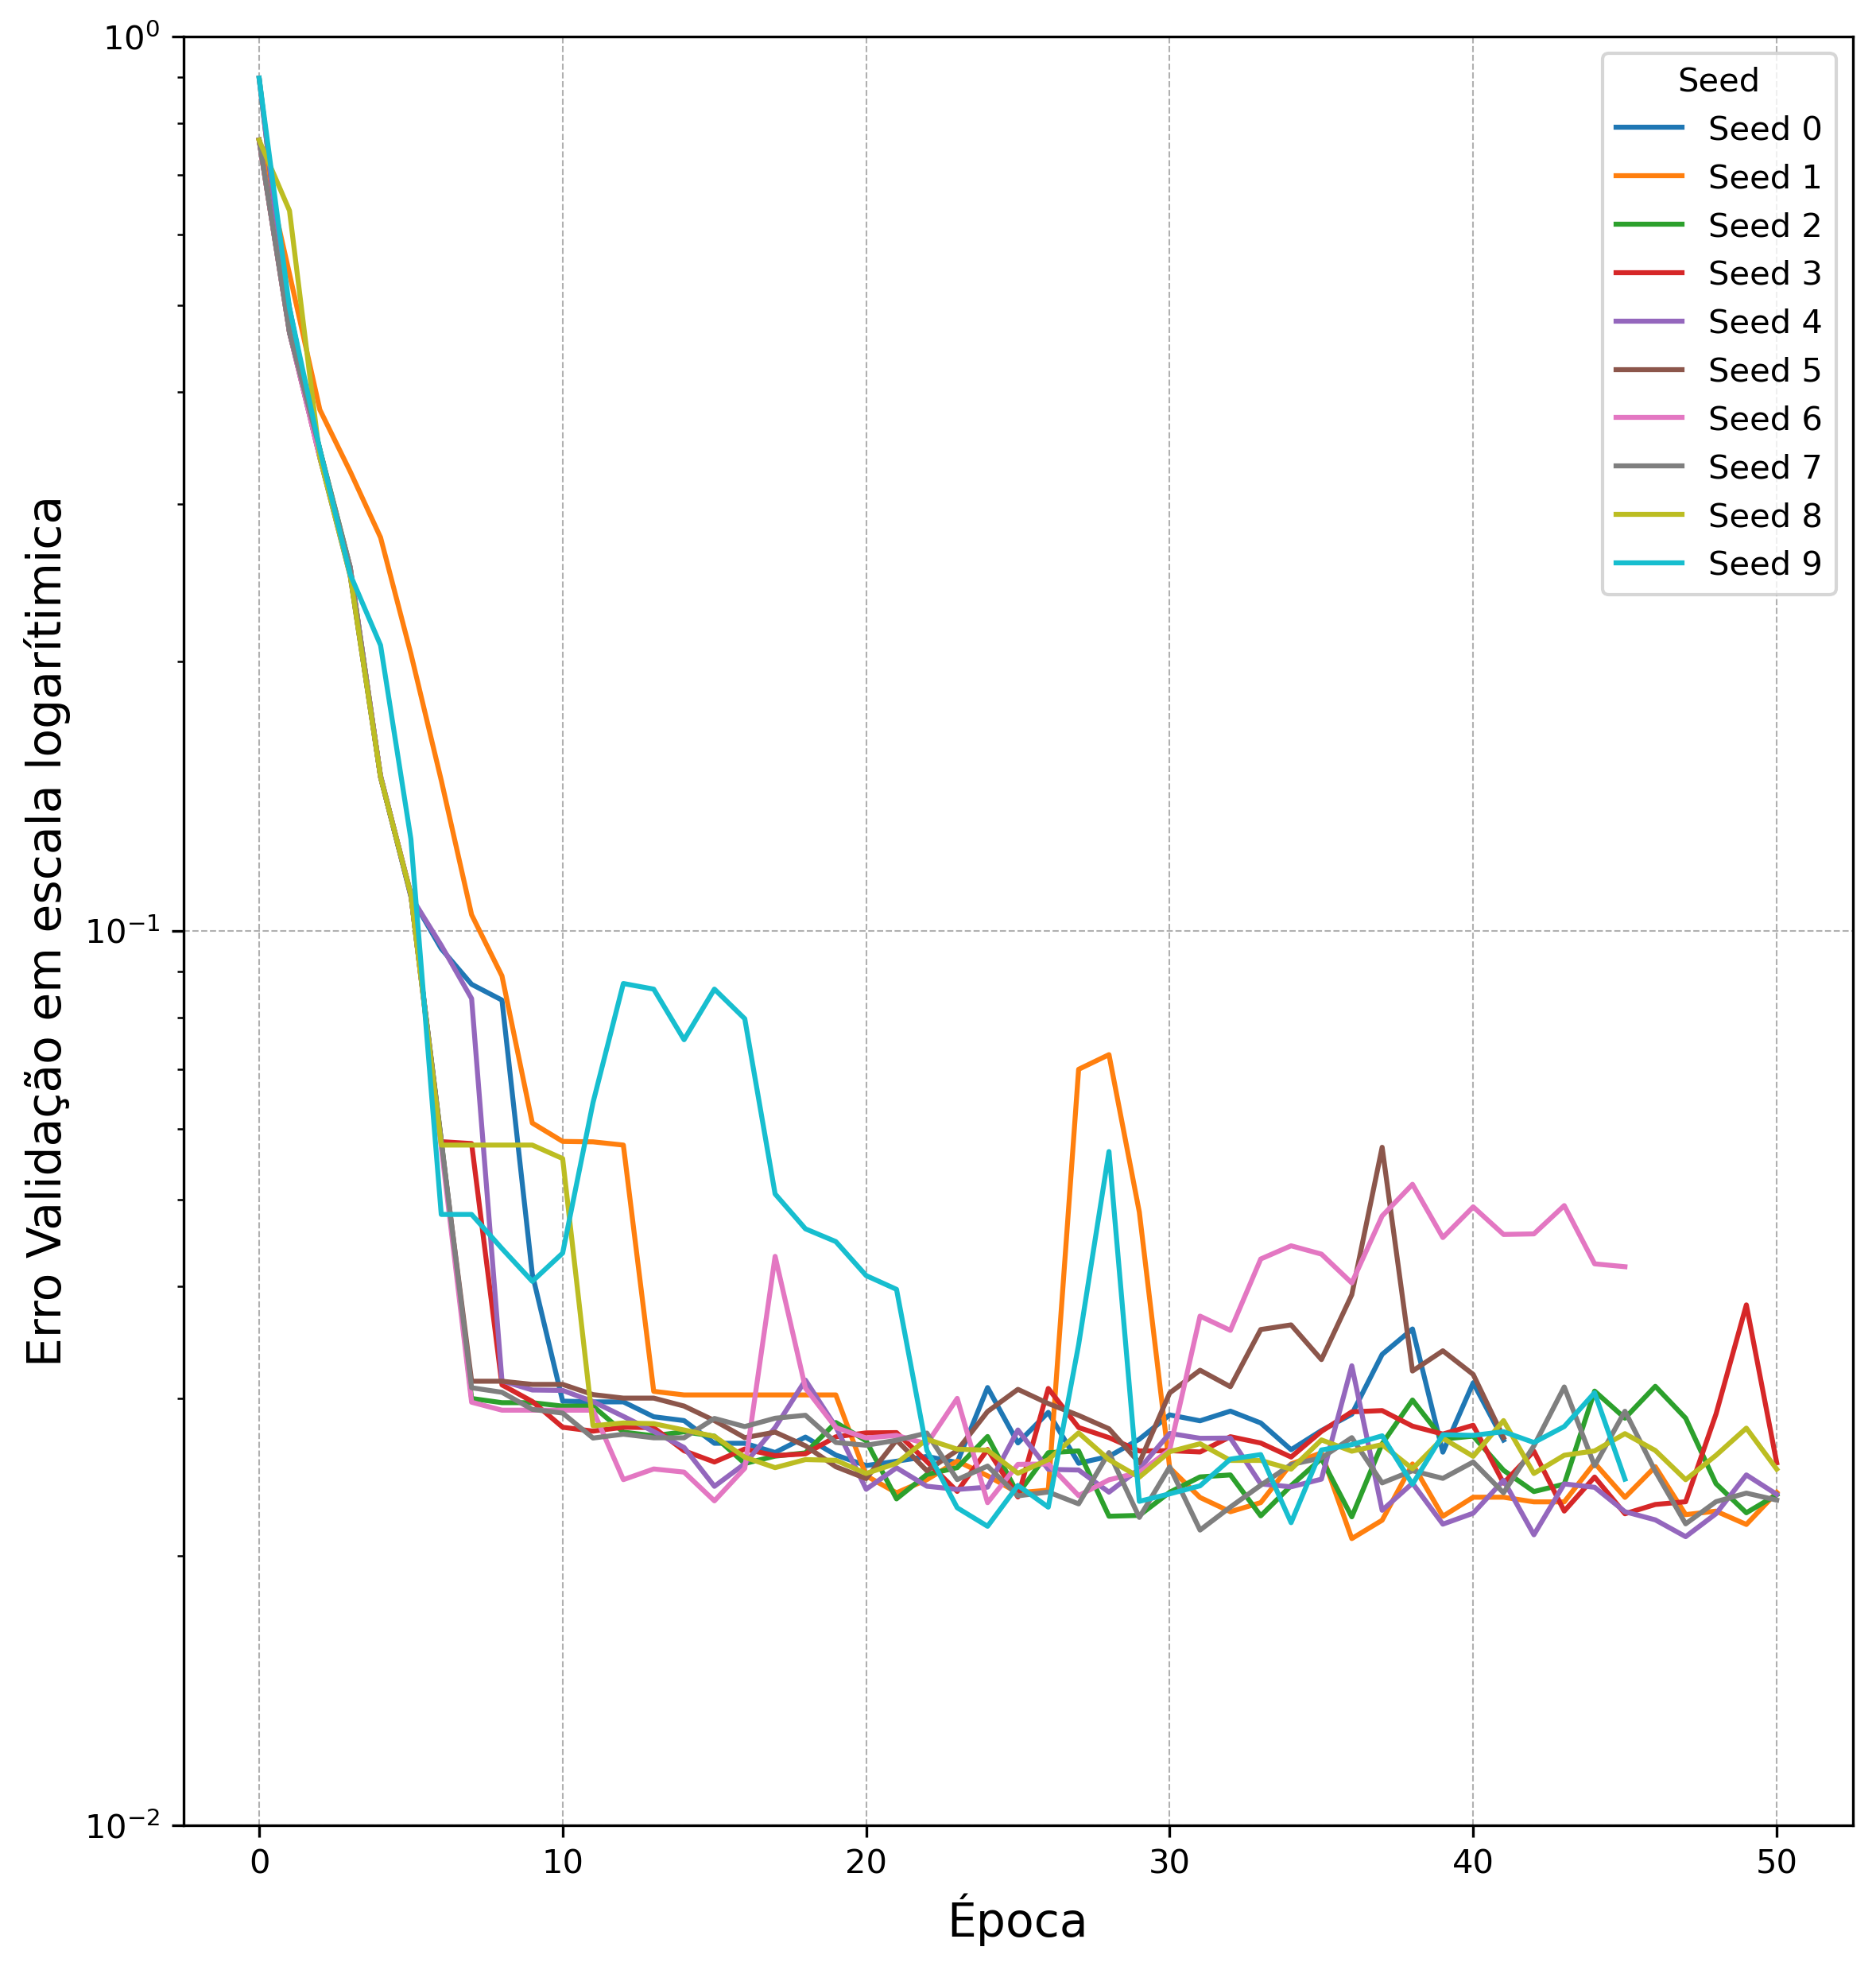
\includegraphics[width=\textwidth]{error_val_plot_25.png}
    \caption{Run 25 - $L_{tt_{mean}}=0.0156$}
  \end{subfigure}

  \caption{Erros de validação ao longo das épocas para as 6 execuções com menor erro médio usando diferentes seeds.\label{fig:validation_errors}}
\end{figure}


Entre todas as execuções, a \textit{Run} 21 - \textit{seed} 1 apresentou o menor erro, com os seguintes resultados: erro de treinamento $L_{t} = 0.0177$, erro de validação $L_{v} = 0.0209$ e erro de teste $L_{tt} = 0.0101$. O tempo total de execução foi de 16.80 minutos, sendo que o erro mínimo foi alcançado na época 36, após 11.25 minutos de processamento. 

Em \cite{DIEGO:DMM}, diversas arquiteturas de redes morfológicas discretas (CDMNN) foram avaliadas com o mesmo conjunto de dados deste experimento, destacando-se a arquitetura \texttt{asf3\_8sg3\_8sg3} com \textit{batch} 5, que apresentou os melhores resultados. Os erros reportados foram de treino $L_{t} = 0.036 - 0.068 \ (0.028)$ e de validação $L_{v} = 0.046 - 0.081 \ (0.025)$, ambos expressos no formato "Valor Mínimo - Valor Médio (Desvio Padrão)". Diferentemente do algoritmo proposto neste trabalho, as CDMNN não utilizam o erro de validação durante o treinamento, sendo o erro de validação equiparado ao erro de teste para fins de comparação. Observa-se que todos os resultados apresentados na Tabela \ref{tab:resultados_runs_digitos} superam o melhor resultado obtido em \cite{DIEGO:DMM}. Em particular, o menor erro de teste obtido, $L_{tt} = 0.0101$, na \textit{Run} 25, é 78\% inferior ao valor mínimo de $0.046$ reportado por \cite{DIEGO:DMM}. Este resultado destaca a superioridade do nosso método para a aplicação em questão.

As imagens de saída após a aplicação em $X$ do primeiro W-operador aprendido nesta execução, são apresentadas na Figura \ref{fig:output_op1}, enquanto o resultado final, após a aplicação dos dois W-operadores, é exibido na Figura \ref{fig:output_op2}. 

Cada camada do W-operador especializou-se em uma tarefa distinta, mesmo sem a imposição de restrições específicas no algoritmo de aprendizado e sendo treinadas em conjunto. A primeira janela foi responsável pela filtragem do ruído sal e pimenta, enquanto a segunda janela realizou a extração das bordas. Esses resultados sugerem que W-operadores podem ter tendência a se especializar na realização de tarefas distintas de forma eficaz, mesmo quando treinados em conjunto, o que implica que camadas distintas em uma arquitetura multicamadas têm a capacidade de se especializar em diferentes tipos de tarefas. Essa observação indica um potencial a ser investigado nos W-operadores em arquiteturas multicamadas, pois cada camada pode se especializar em uma tarefa específica, o que pode levar a um desempenho mais robusto e eficiente. Um fator importante a se considerar é o papel da inicialização dos W-operadores, que pode direcionar o percurso pelos reticulados a diferentes regiões do espaço de soluções, favorecendo a especialização em tarefas distintas.

\begin{figure}
    \centering
    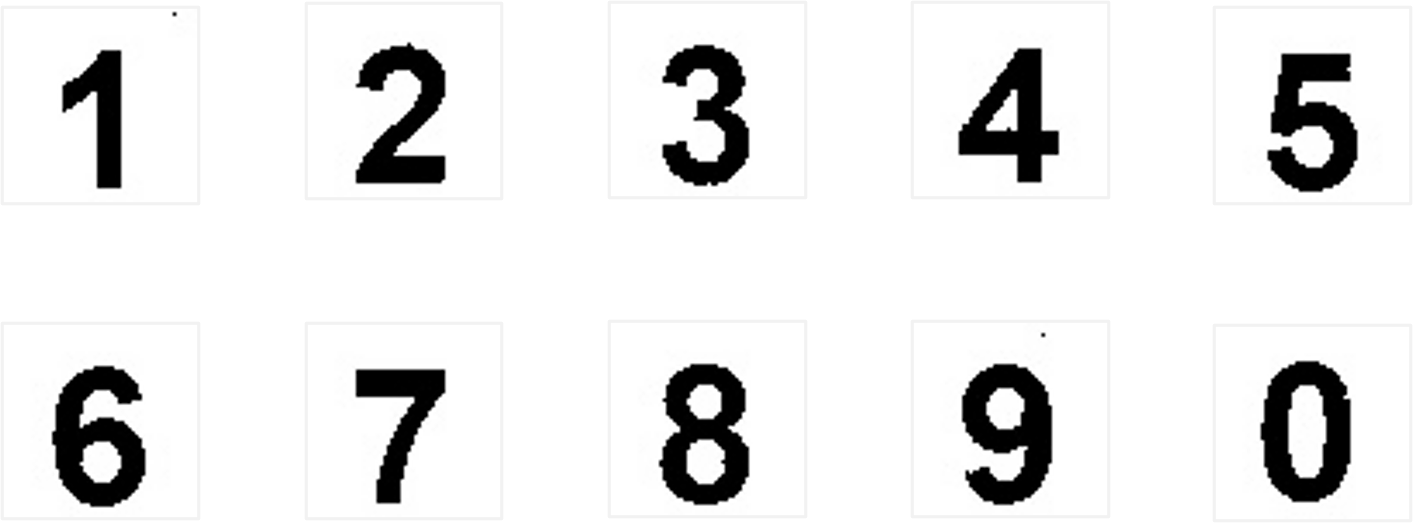
\includegraphics[width=.4\textwidth]{figuras/digitos_output_op1.png}
    \caption{Imagem de saída após aplicar apenas o primeiro W-operador aprendido.}
    \label{fig:output_op1}
\end{figure}


\begin{figure}
    \centering
    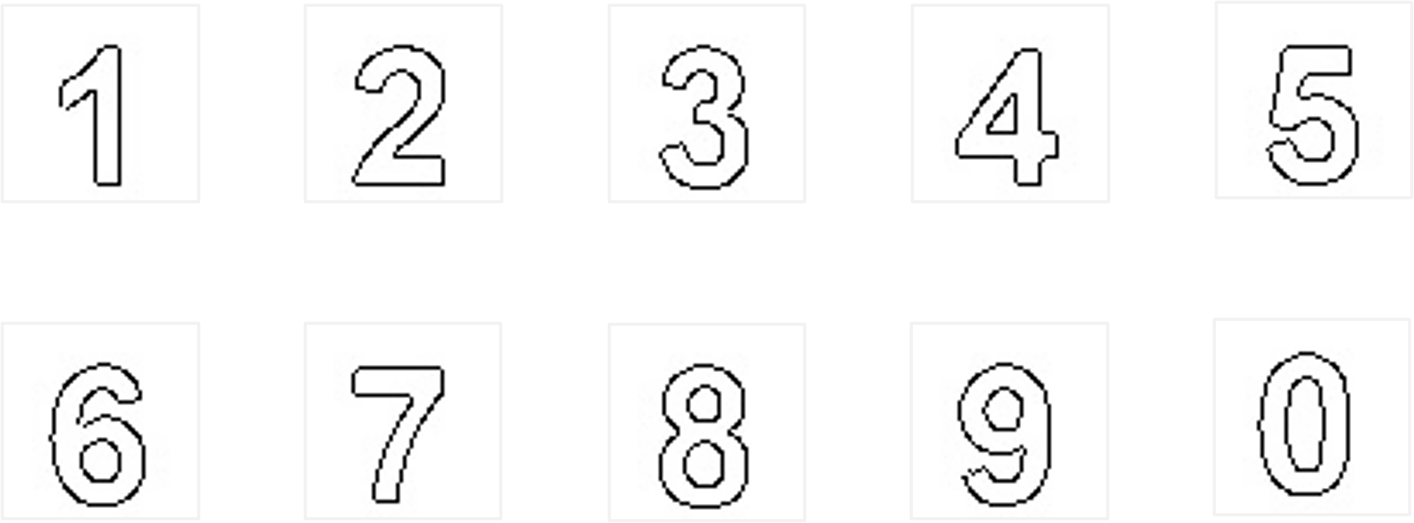
\includegraphics[width=.4\textwidth]{figuras/digitos_output_op2.png}
    \caption{Imagem final de saída após aplicar o WOMC completo aprendido.}
    \label{fig:output_op2}
\end{figure}

Os elementos estruturantes das janelas finais aprendidas pelo algoritmo podem ser observadas na Figura \ref{fig:WOMC}. Nas tabelas \ref{tab:func_w1} e \ref{tab:func_w2} do Apêndice \ref{apsec:reslts_digits} temos as função características completas aprendidas para as duas janelas.

\begin{figure}
  \centering

  \begin{subfigure}{0.4\textwidth}
    \centering
    
\includegraphics[width=.4\textwidth]{figuras/wop_1.png}
    \caption{Janela $W_{1}$\label{fig:subfig:w1}}
  \end{subfigure}
  \begin{subfigure}{0.4\textwidth}
    \centering
      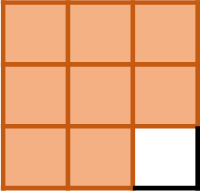
\includegraphics[width=.4\textwidth]{figuras/wop_2.png}
    \caption{Janela $W_{2}$\label{fig:subfig:w1}}
  \end{subfigure}

  \caption{Janelas do WOMC estimadas para realizar a filtragem do ruído sal e pimenta e extração das bordas dos dígitos $0-9$.\label{fig:WOMC}}
\end{figure}

Os resultados obtidos corroboram a afirmação da Introdução \ref{sec:motiv}, já que os resultados representados pelos W-operadores, diferentemente de diversos métodos modernos de aprendizado baseados em redes neurais, são \textbf{interpretáveis}, pois, através do elemento estruturante e funções características dos W-operadores finais de cada camada é possível deduzir matematicamente as propriedades de cada W-operador; e \textbf{possuem consistência lógica, transparência do método e uma boa performance}, uma vez que o erro IoU de 0.0101 é muito baixo, principalmente ao levar em conta que foi utilizada uma amostra de somente 40 imagens para o aprendizado (30 de treino e 10 de validação).

\section{Aprendizado do W-operador de transição do \textit{Conway's Game of Life}}
\label{sec:GoL}

O \textit{Conway's Game of Life} \cite{GOL}, que por simplificação chamaremos a partir de agora de \textbf{GoL}, criado por John Conway em 1970, é um autômato celular que simula a evolução de células em uma grade bidimensional de acordo com um conjunto de regras simples. Cada célula da grade pode estar em um de dois estados possíveis: viva $(1)$ ou morta $(0)$. A evolução do sistema ocorre em passos discretos de tempo, onde o estado de cada célula na próxima geração é determinado por suas células vizinhas, seguindo as seguintes regras:

\begin{itemize}
    \item \textbf{Sobrevivência}: Uma célula viva com dois ou três vizinhos vivos permanece viva na próxima geração.
    \item \textbf{Morte por solidão}: Uma célula viva com menos de dois vizinhos vivos morre, como se fosse por solidão.
    \item \textbf{Morte por superpopulação}: Uma célula viva com mais de três vizinhos vivos morre, devido à superpopulação.
    \item \textbf{Nascimento}: Uma célula morta com exatamente três vizinhos vivos se torna viva, representando o nascimento de uma nova célula.
\end{itemize}

Essas regras fazem com que padrões complexos e dinâmicos emerjam a partir de configurações iniciais simples, tornando o \textbf{GoL} um exemplo clássico de como comportamentos complexos podem surgir de regras simples.

No contexto do nosso experimento, o \textbf{GoL} pode ser visto como uma transformação de imagens, onde as regras do jogo correspondem a um W-operador 3x3 de uma camada, com todos os pontos da janela preenchidos. O W-operador, nesse caso, processa a imagem binária inicial (com células vivas e mortas) para gerar uma nova imagem (o estado seguinte do autômato) com base nas regras pré-definidas.

Esse experimento é particularmente interessante porque o \textbf{GoL} possui uma função de transição conhecida, que é definida precisamente pelas regras do jogo. Essa função está expressa por completo no apêndice \ref{apsec:reslts_gol}. Portanto, podemos avaliar a capacidade do modelo de aprender e replicar um sistema com uma solução exata.

Para aprender a função de transição do \textbf{GoL}, realizamos experimentos utilizando uma configuração com 1 camada ($n=1$) e janelas 3x3 ($d_{W} = 3$). Foram testadas diferentes quantidades de imagens de treinamento ($N = 100 \text{ ou } 300$) e de validação ($M = 100 \text{ ou } 300$) selecionadas aleatóriamente do dataset "GoL\_final", com 16 vizinhos amostrados tanto para a função ($r=16$) quanto para a janela ($s=16$). O aprendizado da função característica ocorreu ao longo de 2000 épocas ($Epoch_f = 2000$) e o aprendizado da janela ao longo de 200 épocas ($Epoch_w = 200$). Utilizou-se um tamanho de batch de 50 ($b=50$), com critério de early stopping para o reticulado da função após 50 épocas ($es_{f} = 50$) e para o reticulado da janela após 10 épocas ($es_{w} = 10$). A janela inicial foi configurada em cruz ($W_{ini} = [[0,1,0],[1,1,1],[0,1,0]]$).

O aprendizado foi realizado com o erro MAE, utilizando diferentes níveis de ruído nas imagens de saída, como segue:

\begin{enumerate}
    \item Imagens de saída originais.
    \item Imagens de saída com 5\% de ruído sal e pimenta.
    \item Imagens de saída com 10\% de ruído sal e pimenta.
    \item Imagens de saída com 15\% de ruído sal e pimenta.
    \item Imagens de saída com 20\% de ruído sal e pimenta.
    \item Imagens de saída com 30\% de ruído sal e pimenta.
\end{enumerate}

A descrição de como o dataset "GoL\_final" foi criado está descrita no apêndice \ref{apsec:reslts_gol}.

O objetivo de incluir o ruído sal e pimenta nas imagens de saída é avaliar se o algoritmo é robusto ao ruído e consegue identificar a função de transição, especialmente em cenários de maior dificuldade, como no caso de 30\% de ruído.

Além do aprendizado tradicional de Janela + Função Característica, foi realizado, para cada um dos cenários, um aprendizado apenas da função, fixando a janela ótima (quadrado 3x3). Nesse caso, não utilizamos a estocasticidade no sorteio dos vizinhos ($r$), realizando uma busca completa no reticulado, com o objetivo de encontrar a função ótima.

Após o término de cada treinamento, os resultados foram comparados com a função de transição já conhecida.

Na Tabela \ref{tab:resultados_gol} , apresentamos os resultados das \textit{Runs} ($R$) de 1 a 12, representando cada um dos experimentos, a coluna $Ruido$ indica o percentual de ruído nesse experimento e a coluna $N$ a quantidade de dados da amostra de treinamento. Em cada experimento tivemos 10 execuções com \textit{seeds} diferentes, ou seja, pontos iniciais diferentes. O cálculo de erro de validação ($L_{v}$) refere-se ao erro durante o processo de validação do aprendizado do algoritmo, apresentado na notação "Valor Mínimo - Valor Médio (Desvio Padrão)" \ calculado sobre as 10 diferentes \textit{seeds} de cada \textit{Run}.

Além disso, a tabela inclui a quantidade de execuções, dentre as 10, em que a função ótima foi aprendida ($P_{f_{ideal}}$) para o aprendizado do algoritmo completo e a quantidade de execuções em que a função ótima foi aprendida ($P_{f_{ideal}-fixed}$) para o aprendizado com janela fixa; Por fim, os percentuais de erro entre a função aprendida e a função de transição conhecida, também para os dois aprendizados sendo denotado por $error_{f_{ideal}}$ e $error_{f_{ideal}-fixed}$, os tempos de aprendizado do algoritmo completo ($t_{total}$) e do algoritmo com janela fixa ($t_{W_{fixed}}$), todos no formato "Valor Mínimo - Valor Médio (Desvio Padrão)".

\begin{table}[ht]
    \centering
    \resizebox{\textwidth}{!}{ % Redimensiona a tabela para caber na largura da página
        \begin{tabular}{ccccccccccc}
            \toprule
            $R$ & $Ruido$ & $N$ & $M$ & $L_{v}$ & $P_{f_{ideal}}$ & $error_{f_{ideal}}$ \ (\%) & $P_{f_{ideal}-fixed}$ & $error_{f_{ideal}-fixed}$ \ (\%) & $t_{total} \ (min)$ & $t_{W_{fixed}} \ (min)$  \\
            \midrule
            1 & 0\%  & 100 & 100 & $0.0015 - 0.0514 \ (0.0492)$ & $0$ & $1.56 - 2.45 \ (0.42)$ &$0$ & $0.20 - 0.39 \ (0.15)$ & $4.10 - 5.98 \ (1.40)$ & $6.55 - 7.26 \ (0.31)$ \\
            2 & 5\%  & 100 & 100 & $0.0681 - 0.1092 \ (0.0418)$ & $0$ & $2.34 - 2.82 \ (0.39)$ & $0$ & $0.20 - 0.39 \ (0.15)$ & $4.00 - 7.91 \ (2.20)$ & $6.61 - 7.03 \ (0.36)$ \\
            3 & 10\% & 100 & 100 & $0.1220 - 0.1617 \ (0.0397)$ & $0$ & $2.34 - 2.93 \ (0.43)$ & $0$ & $0.59 - 0.90 \ (0.20)$ & $3.90 - 7.21 \ (2.55)$ & $7.21 - 8.39 \ (0.67)$ \\
            4 & 15\% & 100 & 100 & $0.1807 - 0.2161 \ (0.0350)$ & $0$ & $2.15 - 3.17 \ (0.52)$ & $0$ & $0.39 - 0.67 \ (0.15)$ & $4.08 - 8.40 \ (2.48)$ & $11.12 - 14.27 \ (2.10)$ \\
            5 & 20\% & 100 & 100 & $0.2429 - 0.2746 \ (0.0319)$ & $0$ & $3.32 - 3.89 \ (0.48)$ & $0$ & $1.37 - 1.57 \ (0.20)$ & $4.28 - 7.07 \ (1.52)$ & $12.89 - 17.20 \ (2.04)$ \\
            6 & 30\% & 100 & 100 & $0.3643 - 0.3866 \ (0.0221)$ & $0$ & $4.49 - 5.49 \ (0.63)$ & $0$ & $8.01 - 9.50 \ (0.92)$ & $4.72 - 6.14 \ (1.05)$ & $11.96 - 23.66 \ (4.68)$ \\
            7 & 0\%  & 300 & 300 & $0.0014 - 0.0516 \ (0.0507)$ & $0$ & $1.76 - 2.25 \ (0.36)$ & $10$ & $0.00 - 0.00 \ (0.00)$ & $9.49 - 16.80 \ (7.81)$ & $3.10 - 3.29 \ (0.10)$ \\
            8 & 5\%  & 300 & 300 & $0.0641 - 0.1104 \ (0.0469)$ & $0$ & $1.56 - 2.56 \ (0.49)$ & $10$ & $0.00 - 0.00 \ (0.00)$ & $9.18 - 14.98 \ (3.44)$ & $3.11 - 3.42 \ (0.19)$ \\
            9 & 10\% & 300 & 300 &  $0.1218 - 0.1654 \ (0.0439)$ & $0$ & $1.56 - 2.53 \ (0.45)$ & $10$ & $0.00 - 0.00 \ (0.00)$ & $9.08 - 15.04 \ (5.66)$ & $3.22 - 3.38 \ (0.12)$ \\
            10 & 15\% & 300 & 300 & $0.1851 - 0.2236 \ (0.0390)$ & $0$ & $1.95 - 2.67 \ (0.58)$ & $10$ & $0.00 - 0.00 \ (0.00)$ & $8.74 - 14.94 \ (4.14)$ & $3.14 - 3.29 \ (0.11)$ \\
            11 & 20\% & 300 & 300 & $0.2479 - 0.2804 \ (0.0344)$ & $0$ & $2.54 - 3.28 \ (0.40)$ &$5$ & $0.00 - 0.10 \ (0.10)$ & $8.85 - 16.25 \ (5.90)$ & $3.08 - 3.26 \ (0.09)$  \\
            12 & 30\% & 300 & 300 & $0.3723 - 0.3969 \ (0.0234)$ & $0$ & $2.73 - 4.31 \ (0.84)$ &$10$ & $0.00 - 0.00 \ (0.00)$ & $8.88 - 15.86 \ (6.69)$ & $3.11 - 3.29 \ (0.10)$ \\
            \bottomrule
        \end{tabular}
    }
    \caption[Resultados das \textit{Runs} \textbf{GoL}]{Resultados das \textit{Runs}, cada uma composta por 10 execuções com \textit{seeds} distintas, variando o nível de ruído nas imagens de saída e os tamanhos das amostras de treino e validação. A tabela apresenta o erros MAE de validação no aprendizado da janela expressos no formato "Valor mínimo - Valor médio (desvio padrão)", quantidade de execuções onde a função de transição foi aprendida e a diferença percentual entre a função característica aprendida e a função de transição no aprendizado da janela,  quantidade de execuções onde a função de transição foi aprendida e diferença percentual entre a função característica aprendida e a função de transição no aprendizado com janela fixa, assim como o tempo total e o tempo gasto no aprendizado com janela fixa, também calculados nas 10 execuções e apresentados no formato "Valor mínimo - Valor médio (desvio padrão)".}
    \label{tab:resultados_gol}
\end{table}





Os resultados obtidos foram altamente satisfatórios. Em todos os cenários testados, o algoritmo demonstrou uma notável capacidade de aprender a janela ideal, mesmo em condições desafiadoras, como no treinamento realizado com apenas 200 imagens e 30\% de erro no dataset. No cenário com menos dados (200 imagens), o aprendizado da função de transição tornou-se mais complexo. Embora o treinamento com uma janela fixa da \textit{Run} 1 ($Ruido = 0\%$, $N=100$ e $M=100$) tenha alcançado erro de treino igual a zero, ao compararmos com a função de transição ideal, observou-se uma diferença de 2 pontos na função característica em todas as seeds. Essa diferença pode ser atribuída ao menor tamanho da amostra, que impediu o algoritmo de capturar todos os exemplos necessários para aprender completamente a função de transição. Esse erro acaba escalonando conforme vamos aumentado o ruído nas imagens de saída, chegando a quase 10\% para o cenário da \textit{Run} 6 ($Ruido = 30\%$, $N=100$ e $M=100$). Importante reparar que o tempo de execução para os treinamentos de janela fixa também são mais elevados, quando comparados ao mesmo treinamento com um conjunto de dados maior, isso decorre pelo algoritmo com mais dados, apesar de demorar mais por época, converge mais rápido.

Por outro lado, no cenário com uma amostra maior (600 imagens), o algoritmo foi capaz de aprender a função característica ideal em praticamente todos os casos. Nas poucas situações em que a função de transição não foi aprendida perfeitamente, apenas 1 dos 512 pontos apresentou divergência, resultando em um erro de teste final médio de apenas 0.0004. Esses resultados evidenciam a eficiência do algoritmo na aprendizagem de um W-operador ótimo. Além disso, o algoritmo mostrou-se robusto ao ignorar o ruído presente no dataset, mantendo a qualidade do aprendizado mesmo sob condições adversas.

\section{WOMC para Classificação com o Dataset MNIST}
\label{sec:mnist}

O dataset MNIST (\textit{Modified National Institute of Standards and Technology}) \cite{MNIST:dataset}, exemplificado na Figura \ref{fig:mnist}, é uma das bases de dados mais utilizadas na área de aprendizado de máquina para avaliar métodos de classificação de imagens. Ele consiste em um conjunto de 70.000 imagens binárias, divididas em 60.000 imagens para treinamento e 10.000 para teste, representando dígitos manuscritos de 0 a 9. Cada imagem possui resolução de 28x28 pixels. A simplicidade e a clareza das imagens, combinadas com sua natureza desafiadora, fazem do MNIST um padrão de referência na validação de algoritmos de classificação.

\begin{figure}
    \centering
    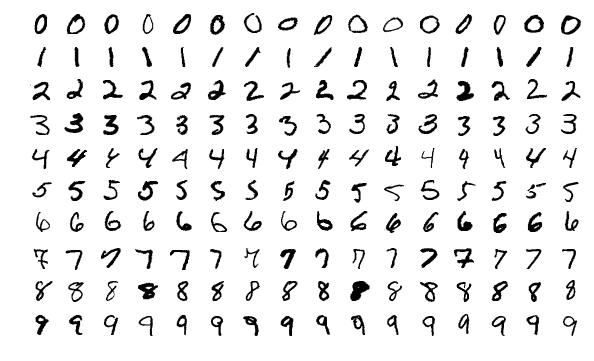
\includegraphics[width=.8\textwidth]{figuras/MNIST_ex.jpg}
    \caption{Amostra de imagens do dataset MNIST. Fonte: \cite{wikipedia_mnist}}
    \label{fig:mnist}
\end{figure}


A importância do MNIST no contexto de aprendizado de máquina reside em sua capacidade de fornecer um benchmark robusto para avaliar o desempenho de algoritmos de classificação. Devido à sua simplicidade relativa, ele permite que pesquisadores e praticantes explorem novas técnicas de aprendizado de forma rápida e eficaz, proporcionando um primeiro passo na avaliação de novos métodos antes de aplicá-los em datasets mais complexos.

O objetivo deste experimento é validar a aplicação do nosso algoritmo no contexto de classificação de imagens utilizando o dataset MNIST. Buscamos demonstrar que o algoritmo é capaz de alcançar um tempo de aprendizado e erro aceitáveis, mesmo quando treinado com um número limitado de imagens. Essa característica é especialmente relevante porque, ao contrário das redes neurais profundas, que apesar de seu poder de generalização, frequentemente exigem grandes quantidades de dados de treinamento e produzem resultados difíceis de interpretar, o método proposto consegue aprender com menos dados e ainda manter a interpretabilidade.

No decorrer deste experimento, pretendemos mostrar que nosso método não só é eficiente, como também mantém um alto nível de interpretabilidade, permitindo uma compreensão clara do processo de decisão. Essa transparência é um dos principais diferenciais da nossa abordagem, tornando-o uma alternativa atraente em cenários onde a explicabilidade do modelo é tão importante quanto sua precisão.

\subsection{Aprendizado do WOMC}

Para avaliar o método no contexto de classificação de imagens, realizamos o aprendizado com foco no dígito 1 utilizando uma configuração com 7 camadas ($n=7$) e janelas 5x5 ($d_{W} = 5$). Podemos ver que este é o experimento de maior complexidade computacional. Para esse experimento utilizamos duas configurações de dados, ambas com baixíssimas quantidade, comparadas ao tamanho total do dataset (60.000 imagens). Primeiro como dados de treinamento mantivemos fixos 100 imagens ($N = 100$), sendo que delas 33 eram o dígito 1 e 67 eram os demais dígitos, selecionado de forma aleatória. Já para os dados de validação para o teste 1 foram selecionadas 100 imagens e para o teste 2, 500 imagens de validação ($M = 100 \ \text{ou} \ 500$), sendo elas 33 ou 100, respectivamente, do dígito 1. A ideia desses experimentos é testar a capacidade de aprendizado com poucos dados, tarefa de maior complexidade quando falamos de redes neurais modernas. O experimento $1b$ com mais imagens de validação consiste em ajudar o algoritmo na seleção da melhor configuração de janelas, quando comparado ao $1a$. 

Os demais parâmetros do algoritmo foram constantes nos dois experimentos: utilizamos 10 vizinhos amostrados para o reticulado das funções características ($r=10$) e 20 vizinhos para o reticulado das janelas ($s=20$); o aprendizado da função característica ocorreu ao longo de 500 épocas ($Epoch_f = 500$) e o aprendizado da janela ao longo de 30 épocas ($Epoch_w = 30$); utilizou-se um tamanho de batch de 50 ($b=50$), com critério de early stopping para o reticulado da função após 50 épocas ($es_{f} = 50$) e para o reticulado da janela após 10 épocas ($es_{w} = 10$). A janela inicial foi configurada em cruz ($W_{ini} = [[0,0,0,0,0],[0,0,1,0,0],[0,1,1,1,0],[0,0,1,0,0],[0,0,0,0,0]]$).

%Apesar da baixíssima quantidade de dados, atingimos erro de treino $L_{t} = 0.0100$ e de validação de $L_{v} = 0.0100$ na época 26 após 440 minutos. O treino total ficou em 653 minutos e o erro no dataset completo de teste do MNIST (10.000 imagens) ficou em $L_{tt} = 0.0762$.

Os resultados desses experimentos encontram-se na Tabela \ref{tab:resultados_mnist} onde os erros de teste ficaram em 0.0762 para a \textit{Run} 1 e 0.0317 para a \textit{Run} 2. Resultados acima da expectativa dada a baixa quantidade de dados de treinamento e a baixa quantidade de épocas utilizadas.

A Figura \ref{fig:confusion_matrix}  apresenta as matrizes de confusão obtida após o treinamento utilizando os dados de teste. Esta matriz é uma ferramenta essencial para avaliar a performance do modelo de classificação, indicando como as previsões se alinham com os valores reais.

Na matriz, o campo \textbf{Verdadeiros Negativos (0,0)} mostra que 97\% dos exemplos que não representam o dígito 1 foram corretamente classificados como não sendo o dígito 1 no experimento 2 e 93\% no experimento 1. O campo \textbf{Falsos Positivos (0,1)} indica que 3\% desses exemplos foram incorretamente classificados como o dígito 1 no experimento 2 e 7\% no experimento 1. Já o campo \textbf{Falsos Negativos (1,0)} revela que 4\% dos exemplos que representam o dígito 1 foram incorretamente classificados como não sendo o dígito 1 no experimento 2 e 9\% no experimento 1. Por fim, o campo \textbf{Verdadeiros Positivos (1,1)} mostra que 96\% dos exemplos do dígito 1 foram corretamente identificados como o dígito 1 no experimento 2 e 91\% no experimento 1.

Esses resultados indicam que mesmo com uma baixíssima quantidade de dados, o modelo possui alta precisão na identificação do dígito 1, com baixas taxas de erro, o que demonstra sua eficácia na tarefa de classificação.

\begin{figure}
  \centering

  \begin{subfigure}{0.49\textwidth}
    \centering
    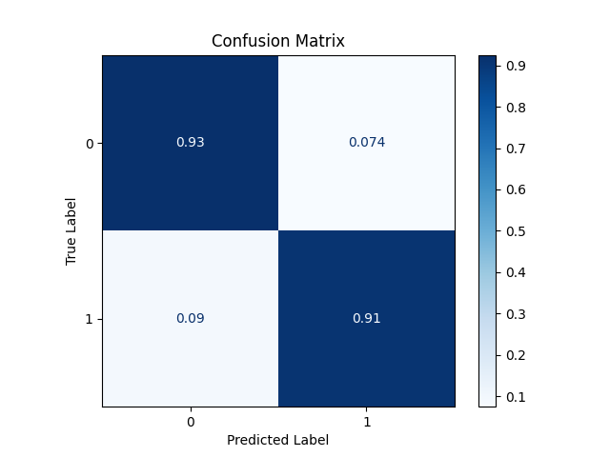
\includegraphics[width=1.1\textwidth]{figuras/conf_matrix_100.png}
    \caption{Matriz de confusão do experimento $1$ ($M=100$).\label{fig:subfig:conf1}}
  \end{subfigure}
  \begin{subfigure}{0.49\textwidth}
    \centering
      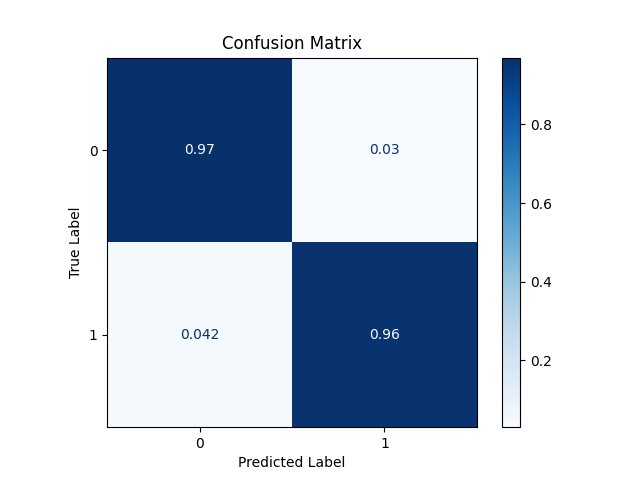
\includegraphics[width=1.1\textwidth]{figuras/conf_matrix.png}
    \caption{Matriz de confusão do experimento $2$ ($M=500$)\label{fig:subfig:conf2}}
  \end{subfigure}

  \caption{Matriz de Confusão para os experimentos de aprendizado do WOMC no contexto de classificação do dígito 1.\label{fig:confusion_matrix}}
\end{figure}

Nas Figuras \ref{fig:painel_acerto} e \ref{fig:painel_erro}, podemos observar o comportamento do W-operador final aprendido, analisando seu funcionamento em cada camada e o resultado final, com o último bit correspondente à classificação. A Figura \ref{fig:painel_acerto} exibe o painel dos acertos, enquanto a Figura \ref{fig:painel_erro} apresenta o painel dos erros. A partir da análise detalhada de cada W-operador em cada camada e dos resultados representados nesses painéis, é possível inferir o processo de classificação do modelo. Esta etapa é crucial para avaliar a interpretabilidade do modelo, permitindo compreender como as decisões de classificação estão sendo tomadas.

\begin{figure}[H]
    \centering
    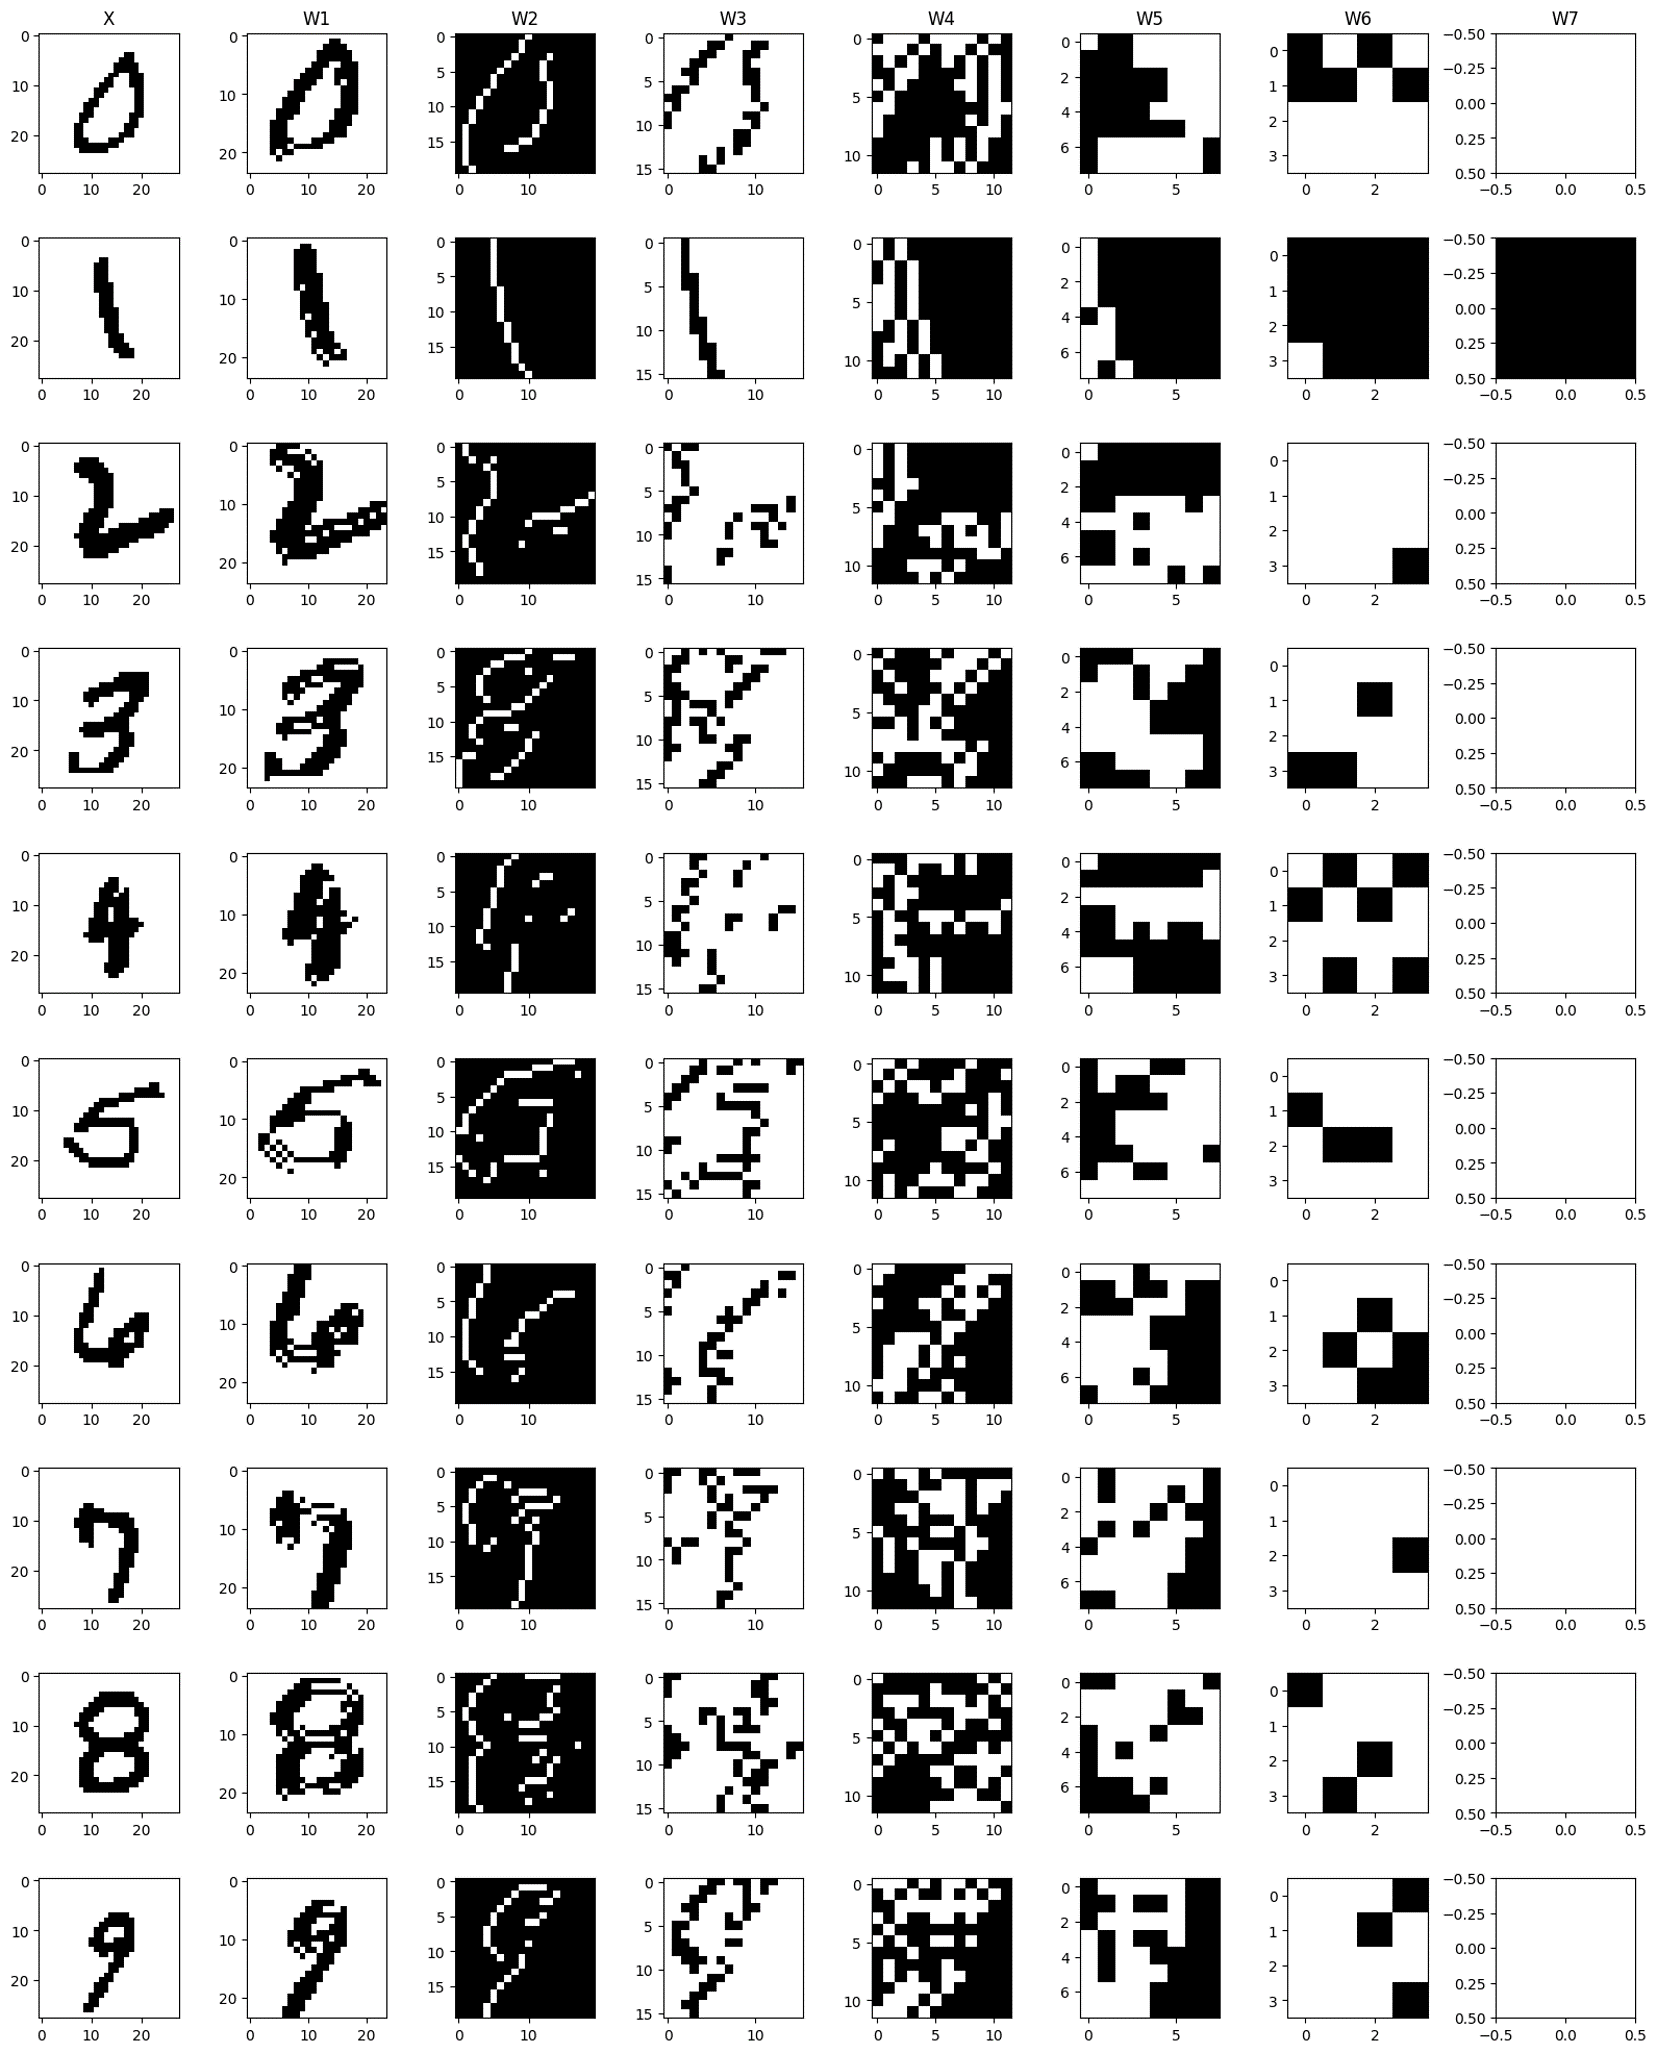
\includegraphics[width=0.5\textwidth]{figuras/painel_acerto.png}
    \caption{Painel de imagens classificadas corretamente.}
    \label{fig:painel_acerto}
\end{figure}

\begin{figure}[H]
    \centering
    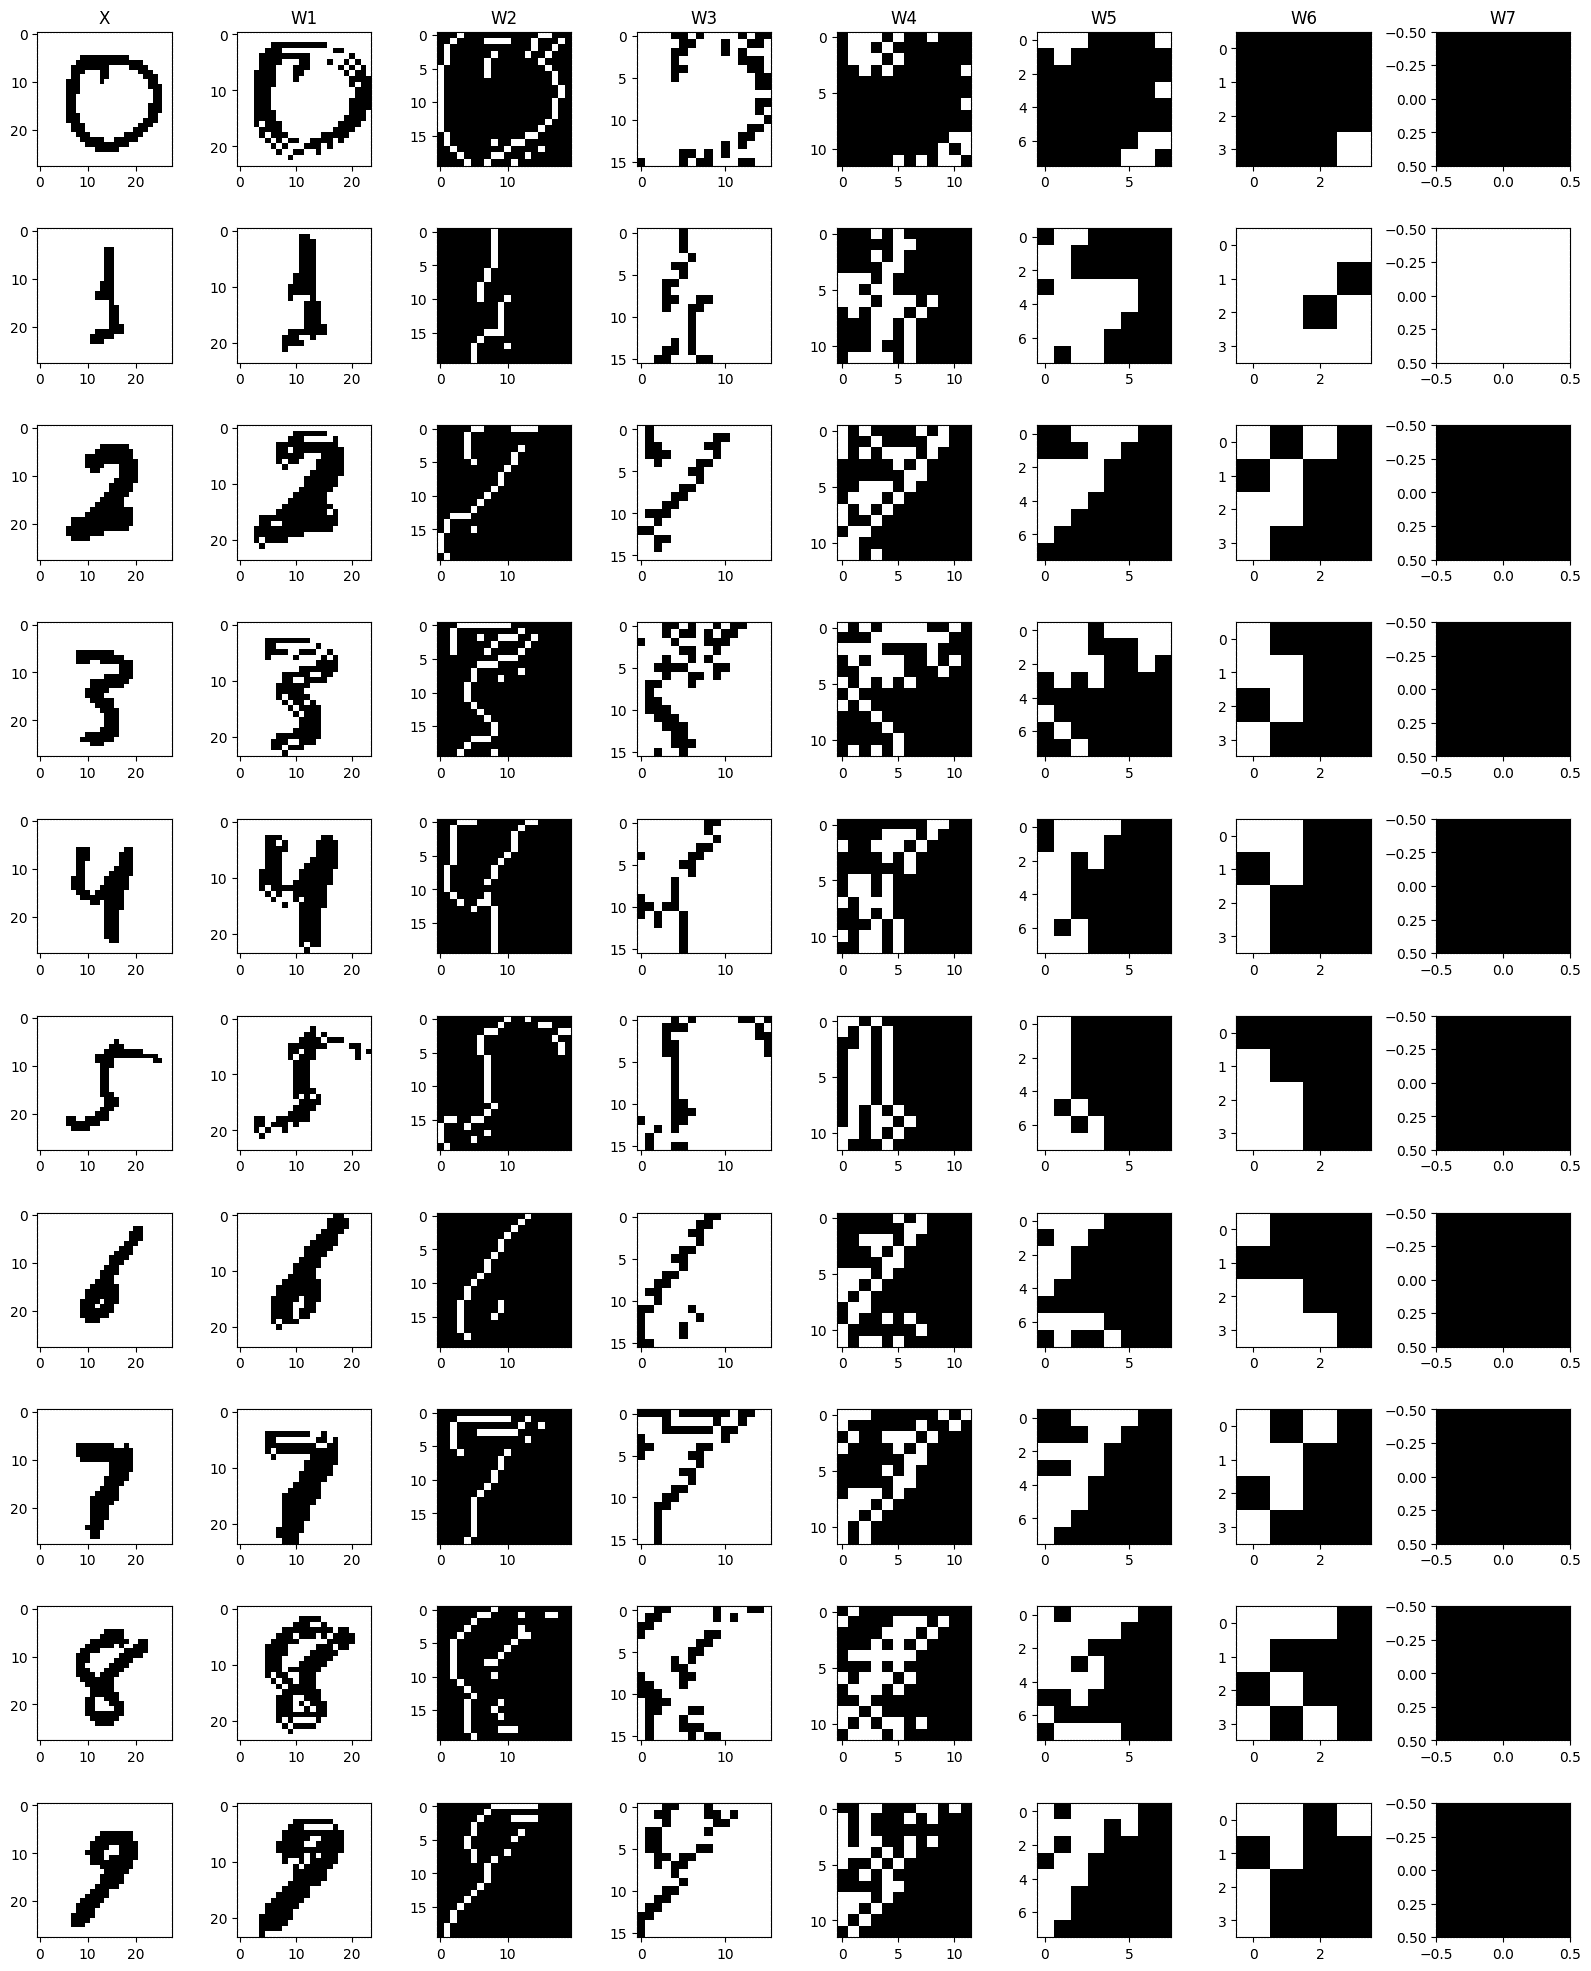
\includegraphics[width=0.5\textwidth]{figuras/painel_erro.png}
    \caption{Painel de imagens classificadas incorretamente.}
    \label{fig:painel_erro}
\end{figure}

\subsection{Aprendizado com Rede Neural}

Para fins de comparação, treinamos o conjunto de dados MNIST utilizando uma rede neural convolucional (CNN) para a tarefa de classificação de imagens. A descrição completa da configuração dessa rede encontra-se no Apêndice \ref{apsec:cnn}.  (\textit{early stop} = quantidade de épocas).

Na primeira parte do experimento, seguimos a metodologia tradicional, utilizando todas as 60.000 imagens de treino e avaliando o erro nas 10.000 imagens do conjunto de teste. Com um batch size de 256 e apenas 10 épocas de treinamento, a rede neural alcançou um erro no conjunto de teste de 0.0015, como esperado para esse tipo de modelo. Esse teste foi realizado para comprovar a eficiência da arquitetura utilizada para a comparação

Na segunda parte do experimento temos o objetivo de comparar os métodos WOMC e CNN. A arquitetura da CNN utiliza dados de validação não durante o treinamento, mas como critério de \textit{early stop}, para garantir a justa comparação entre os métodos utilizamos sempre a quantidade de amostra de treinamento igual a soma da amostra de treino e validação no método WOMC e removemos o critério de \textit{early stop}. Foram realizados 2 experimentos então, as \textit{Runs} 3 e 4 a serem comparadas com as \textit{Runs} 1 e 2, com as mesmas 200 e 600 imagens treinadas nos experimento do WOMC, respectivamente. O experimento foi realizado com 100 épocas de treinamento e \textit{batch} de 50. O erro final no conjunto de teste foi de 0.8857 para a \textit{Run} 3 e de 0.0043 para a \textit{Run} 4, evidenciando que a rede neural não conseguiu aprender e generalizar de forma eficiente com a arquitetura empregada, especialmente com a quantidade limitada de apenas 200 imagens. Em contraste, ao utilizar 600 imagens, a CNN demonstrou uma capacidade de generalização superior em comparação ao método WOMC.

\subsection{Resultados}

A tabela \ref{tab:resultados_mnist} apresenta os resultados compilados dos experimentos mencionados acima com o aprendizado do WOMC nos experimentos 1 e 2 com $M=100$ e $M=500$ respectivamente e dos experimentos com a CNN nos experimentos 3 e 4 com $N=200$ e $N=600$.

\begin{table}[ht]
    \centering
    \resizebox{\textwidth}{!}{ % Redimensiona a tabela para caber na largura da página
        \begin{tabular}{cccccccccc}
            \toprule
            $R$ & Método & $N$ & $M$ & $L_{t}$ & $L_{v}$ & $L_{tt}$ & $Epoch_{W_{min}}$ & $t_{total} \ (min)$ & $t_{Epoch_{min}} \ (min)$ \\
            \midrule
            1 & WOMC & 100 & 100 & 0.0100 & 0.0100 & 0.0762 & 26 & 653 & 440 \\
            2 & WOMC & 100 & 500 & 0.0050 & 0.0180 & 0.0317 & 21 & 792 & 473 \\
            3 & CNN  & 200 & 100 & 0.6700 & 0.6600 & 0.8865 & 55 & 2 & 4 \\
            4 & CNN  & 600 & 100 & 0.0117 & 0.0500 & 0.0043 & 63 & 6 & 10 \\
            \bottomrule
        \end{tabular}
    }
    \caption[Resultados dos experimentos MNIST Dataset]{Resultados dos experimentos para a classificação do dígito 1, utilizando os métodos WOMC e CNN, com as diferentes configurações de tamanho de dataset de treino e validação. São apresentados os erros de treino, validação e teste, a época com erro de validação mínimo, o tempo total e o tempo para o erro de validação mínimo.}
    \label{tab:resultados_mnist}
\end{table}